\documentclass[12pt]{article}
\usepackage[utf8]{inputenc} % кодировка utf8
\usepackage{mathtext} % кириллица в формулах \text{}
\usepackage{amsmath} % пробелы между слов в \text{}
\usepackage[english,russian]{babel}
\usepackage{indentfirst} % красная строка
\usepackage{graphicx} % отображение картинок
\usepackage{subfigure} % отображение коллажа картинок
\usepackage{amssymb} % отображение математической нотации
\usepackage{multirow} % для разделения строк в таблицах
\usepackage{hhline} % для таблиц \hhline{...}
\usepackage{array} % для таблиц m{...}
\usepackage[table]{xcolor} % раскраска ячеек таблицы
\usepackage[nottoc,notlot,notlof]{tocbibind} % для отображения списка литературы в содержании
\usepackage{setspace} % интервал между строк
\usepackage[
    left=30mm, right=20mm,
    top=20mm, bottom=20mm,
    bindingoffset=0mm
    ]{geometry} % настройка границ документа
\usepackage{fancyhdr}



\begin{document}

    \def\figurename{Рисунок}  % "Рис. N" --> "Рисунок N:"

    \begin{titlepage}
        \onehalfspacing
        \begin{center}
            \begin{figure}[h]
                \centering
                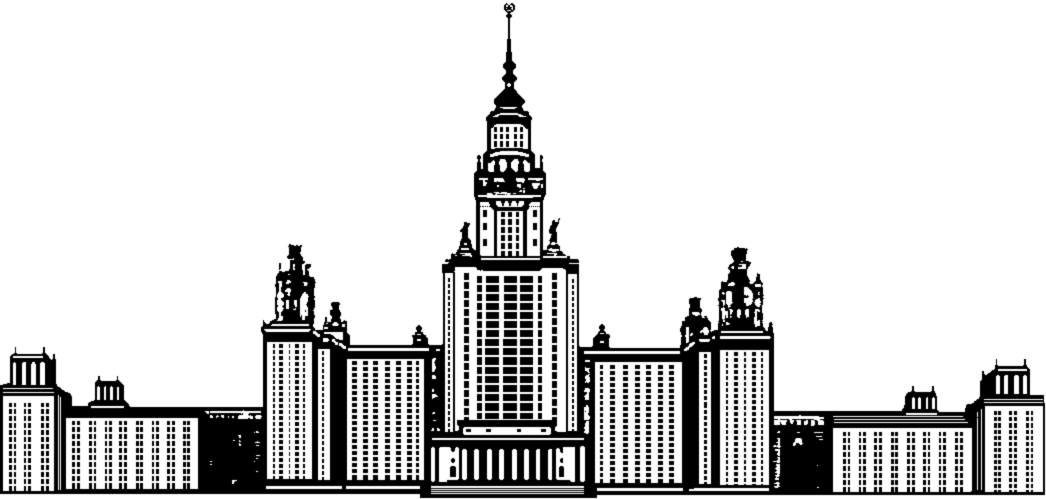
\includegraphics[width=0.4\linewidth]{MSU_logo.png}
            \end{figure}

            Московский государственный университет имени М.В. Ломоносова \\
            Факультет вычислительной математики и кибернетики \\
            Кафедра интелектуальных информационных технологий

            \vfill

            {\large Березникер Алексей Витальевич} \\
            \vspace{5mm}

            {\Large \textbf{
            Динамическая аутентификация пользователей \\
            на основе анализа работы с компьютерной мышью
            }} \\
            \vspace{15mm}

            КУРСОВАЯ РАБОТА \\

            \vfill

            \begin{flushright}
                \textbf{Научный руководитель:} \\
                кандидат физико-математических наук, \\
                математик М.А. Казачук \\
            \end{flushright}
            \vfill

            Москва, 2020 г.
        \end{center}
    \end{titlepage}

    \setcounter{page}{2}  % Титульный лист включается в нумерацию, но не нумеруется

    \tableofcontents
    \newpage


    \onehalfspacing % полуторный интервал


    \section{Аннотация}
    \label{sec:Annotation}

    \par Целью данной работы является исследование существующих и разработка собственных алгоритмов динамической аутентификации пользователя на основе анализа работы с компьютерной мышью, показывающих высокое качество работы и способных работать в динамическом режиме. В работе рассматриваются существующие методы динамической аутентификации, основанные на использовании классических методов машинного обучения и нейронных сетей, а также способы построения и предобработки признакового пространства. Анализируются достоинства и недостатки различных подходов.

    \par Мы фокусируемся на независимой от контекста системе динамической аутентификации, которая реагирует на каждое отдельное действие, выполненное пользователем.

    \par Отметим, что динамическая аутентификация не является альтернативным решением безопасности для первоначального входа в систему, она обеспечивает дополнительную меру безопасности наряду с первоначальным логином.

    \newpage



    \section{Введение}
    \label{sec:Intro}

    \subsection{Область применения}
    \label{sec:Intro:ApplicationArea}

    \par В настоящее время неотъемлемой частью различных сфер деятельности человека стало использование информационных систем. Огромное количество информации ограниченного доступа переносится, хранится и обрабатывается в информационных системах, что формирует потребность в обеспечении их защищенности.

    \par Люди используют механизмы контроля доступа, такие как пароль, магнитные карты или биометрию для защиты от несанкционированного доступа другого человека. Это означает, что пользователь должен предоставить подтверждение своей личности при запуске или разблокировке системы. Однако во многих случаях люди оставляют компьютер без присмотра, временно покидая свое рабочее место, просто потому что у них отсутствует привычка выключать компьютер.

    \par Контроль доступа к персональному компьютеру (ПК) обычно реализуется как единоразовое подтверждение личности во время первичной авторизации. Предполагается, что в течении всего сеанса в системе будет находиться зарегистрированный пользователь. К сожалению, когда компьютер оставлен без присмотра, любой человек может получить доступ к тем же источникам данных, что и легитимный пользователь.

    \par Защита информации в информационных системах обеспечивается созданием комплексной системы защиты, одной из главных составляющих которой являются методы защиты от несанкционированного доступа \cite{BiometricRecognition, BiometricSystem}.

    \par Основой программно-технических средств защиты от несанкционированного доступа являются процедуры идентификации и аутентификации пользователей. Идентификатором в таком случае служит уникальный признак объекта, позволяющий отличить его от других объектов. А под процедурой аутентификации подразумевается процесс проверки принадлежности субъекту доступа предъявленного им идентификатора.


    \subsection{Методы аутентификации}
    \label{sec:Intro:ApplicationArea:AuthenticationMethods}

    \par Существующие методы осуществления аутентификации можно разделить на три категории:

    \begin{enumerate}
        \item методы, основанные на обладании субъекта аутентификации некоторым секретным знанием. В качестве такого знания может выступать секретное слово, пароль или цифровой сертификат. Данный метод является самым распространенным и простым, поэтому он часто подвержен успешным атакам со стороны злоумышленников.

        \item методы, основанные на наличии у субъекта идентификации некоторого физического объекта. Таким объектом может быть, например, ключ, флеш-накопитель или магнитная карта. Аутентификация по предъявлении чего-либо, чем владеет пользователь, имеет сходные недостатки с предыдущей категорией, и, кроме того, добавляется риск передачи, утери, кражи или копирования ключа. Также требуется специальное оборудование для распознавания идентификатора, используемого при аутентификации.

        \item методы, основанные на собственных свойствах субъекта доступа. В качестве таких свойств могут рассматриваться биометрические данные пользователя, т.е. уникальные биологические и физиологические характеристики, которые позволяют установить личность человека. Методы аутентификации, основанные на проверке подлинности через предъявление биометрического образа называются биометрической аутентификацией.
    \end{enumerate}


    \par Существующие в настоящее время методы биометрической аутентификации могут быть основаны на физиологических характеристиках человека, находящиеся при нем в течение всей его жизни, или поведенческих характеристиках человека, являющихся характеристиками поведения индивидума и отличающихся относительной устойчивостью и постоянством проявления. Данные методы разделяются на два класса:

    \begin{enumerate}
        \item \textsc{Статические методы биометрической аутентификации} \\
        Статическая аутентификация заключается в эпизодической проверке личности пользователя (например, при его входе в систему), после чего, в случае успешного прохождения, предоставляется доступ к системе. Например, проверка отпечатка пальца, сетчатки глаза или геометрии лица.

        \item \textsc{Динамические методы биометрической аутентификации} \\
        Динамическая аутентификация предполагает проведение проверки личности пользователя постоянно -- на протяжении всей сессии. Например, анализ голоса, клавиатурного почерка или работы с компьютерной мышью. Под <<клавиатурным почерком>> понимаются характеристики динамики работы пользователя с клавиатурой компьютера.
    \end{enumerate}

    \par Основным недостатком методов проверки пользователей, основанных на физиологической биометрии, является то, что они требуют наличия аппаратных устройств, таких как датчики отпечатков пальцев и сканеры сетчатки, которые дороги и не всегда доступны. Хотя проверка отпечатков пальцев становится широко распространенной в ноутбуках и смартфонах, она все еще недостаточно популярна и не может быть использована в веб-приложениях. Кроме того, отпечатки пальцев могут быть скопированы.

    \par В свою очередь методы, основанные на поведенческой биометрии не требуют специального оборудования, так как они используют обычные устройства ввода, такие как мышь и клавиатура, для сбора биометрических данных.

    \par Другим важным отличием между физиологической и поведенческой биометрией является временной аспект. Поведенческая биометрия может отличаться в зависимости от режима работы пользователя и времени суток, когда она была зафиксированна. Это усложняет процесс подражания для обхода системы, даже в случае перехвата части данных.

    \par Очевидно, динамическая аутентификация пользователей является предпочтительней, так как она исключает сценарии, при которых злоумышленник получает доступ к информационной системе после того, как легитимный пользователь пройдет процедуру аутентификации. Однако данный подход затрачивает больше ресурсов компьютера, за счет непрерывной работы.


    \subsection{Актуальность}
    \label{sec:Intro:Relevance}

    \par Таким образом, мы видим проблемы отсутствия контроля факта смены пользователя и компрометации идентификаторов, которые мы предлагаем решить использованием биометрических поведенческих характеристик пользователя для динамической аутентификации.

    \par Достоинство нашего подхода заключается в простоте внедрения: нужно лишь устройство ввода (компьютерная мышь) и специальное программное обеспечение, позволяющее проводить анализ.

    \newpage



    \section{Постановка задачи}
    \label{sec:FormulationOfProblem}

    \par Задачей данной работы является исследование существующих и разработка собственных алгоритмов динамической аутентификации пользователя на основе анализа работы с компьютерной мышью, показывающих высокое качество работы и способных работать в динамическом режиме. А также исследование методов построения и предобработки признаковых простраснтв.

    \par Наше решение должно выполнять задачи незаметно для пользователя, выявлять злоумышленника как можно быстрее, в то же время избегая в максимально возможной степени неправильной блокировки легитимного пользователя.

    \newpage



    \section{Обзор существующих решений}
    \label{sec:Overview}

    \subsection{Цели обзора}
    \label{sec:Overview:Goals}

    \par Целями данного обзора являются:

    \begin{enumerate}
        \item изучение показателей эффективности биометрических систем;
        \item выявление достоинств и недостатков существующих подходов;
        \item выявление наиболее релевантных признаков для построения модели пользователя;
        \item выявление методов построения модели пользователя, показывающие наилучшее качество аутентификации;
        \item поиск открытых наборов данных для проведения собственных исследований;
        \item формулировка направлений дальнейших исследований.
    \end{enumerate}


    \subsection{Показатели эффективности}
    \label{sec:Overview:Metrics}

    \par Согласно \cite{BiometricRecognition, BoiometricSecurity}, решение об аутентификации должно основываться на результате процесса сопоставления вновь представленных биометрических данных с предварительно сохраненными эталонными шаблонами. Основными метриками оценки качества работы системы аутентификации являются:

    \begin{itemize}
        \item \textsc{Коэффициент ложных отклонений} \\
        Коэффициент ложных отклонений (FRR: False Rejection Rate) -- это доля случаев, когда биометрическая система не предоставляет доступ легитимному пользователю. В статистическом смысле, FRR -- это ошибка I рода. FRR также известен как частота ложных несовпадений (FNMR: False Non Match Rate).

        \item \textsc{Коэффициент ложного принятия} \\
        Биометрическая безопасность использует коэффициент ложного принятия (FAR: False Acceptance Rate) для доли случаев, когда система предоставляет доступ неуполномоченному лицу. С точки зрения статистики, FAR -- это ошибка II рода. Этот коэффициент также известен как частота ложных совпадений (FMR: False Match Rate).

        \item \textsc{Равный коэффициент ошибок} \\
        Одним из основных способов обобщить рабочие характеристики биометрической системы безопасности является рассмотрение коэффициента переходных ошибок (CER: Crossover Error Rate), также известного как равный коэффициент ошибок (EER: Equal Error Rate). Это состояние, при котором ошибки FAR и FRR равны. EER дает возможность сравнивать системы. Чем меньше EER, тем лучше. Меньшее значение EER означает, что можно настроить систему так, чтобы частота ошибок как для I рода, так и для II рода была меньше.
    \end{itemize}

    \par В приложениях безопасности FAR (неавторизованный доступ) хуже, чем FRR (блокировка авторизованного пользователя). Первое может привести к нарушению конфидециальности данных, а второе станет лишь неудобством. Конечно, может быть ситуация, в которой последствия FAR и FRR равны или что FRR хуже, но обычно это не так.
    \vspace{5mm}
    \begin{figure}[h!]
        \centering
        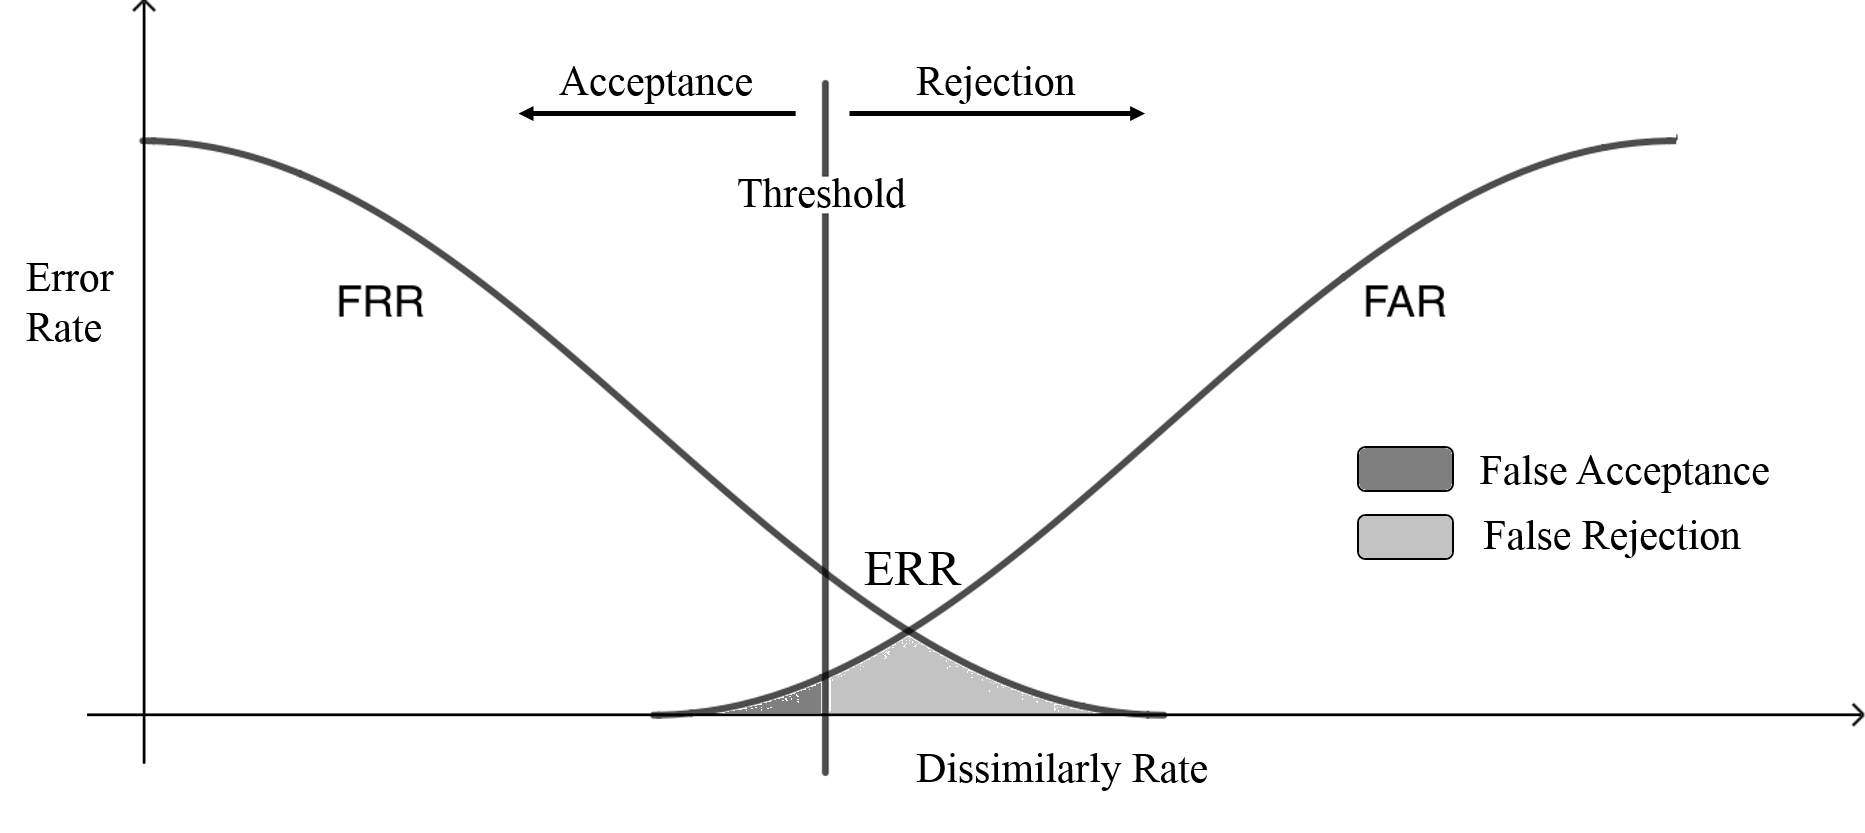
\includegraphics[width=\linewidth]{FAR_FRR_ERR.png}
        \caption{Графическая интерпретация FAR, FRR и EER}
        \label{sec:Overview:Metrics:fig:FAR_FRR_EER}
    \end{figure}

    \begin{itemize}
        \item \textsc{Рабочая характеристика системы} \\
        Рабочая характеристика системы (ROC: Receiver operating characteristic) или ROC-кривая -- это график компромисса между характеристиками FAR и FRR. В общем случае алгоритм принимает решение на основе порогового значения, которое определяет, насколько близко к эталону должен быть вход, чтобы его можно было считать совпадающим. Если порог уменьшится, будет меньше ложных отклонений, но больше ложных принятий. И наоборот, более высокий порог уменьшит FAR, но увеличит FRR. Качество оценивают как площадь под ROC кривой (ROC AUC: Area Under ROC Curve).
    \end{itemize}

    \par Значения метрик EER и ROC-AUC являются основными показателями эффективности для сравнения качества работы различных систем аутентификации, именно их используют в большинстве статей обзора [7 -- 19].

    \par Однако авторы ряда публикаций \cite{Mondal, Mondal_2, Mondal_3} верно заметили, что для системы, на самом деле, важно знать не только об обнаружении нарушителя, но и когда было совершено внедрение, т.е. сколько действий нарушитель был в состоянии совершить до обнаружения. Поэтому они предложили использовать следующие характеристики для оценки эффективности работы системы:

    \begin{itemize}
        \item \textsc{Среднее количество действий злоумышленника} \\
        Среднее количество действий злоумышленника (ANIA: Average Number of Imposter Actions) показывает, сколько действий успеет совершить нарушитель до того момента, как он будет заблокирован системой.
        \item \textsc{Среднее количество легитимных действий} \\
        Среднее количество легитимных действий (ANGA: Average Number of Genuine Actions) характеризует количество действий авторизованного пользователя до его ошибочной блокировки системой.
    \end{itemize}

    \par В данных терминах система будет обладать лучшими качествами при минимизации ANIA и максимизации ANGA.

    \begin{figure}[h!]
        \centering
        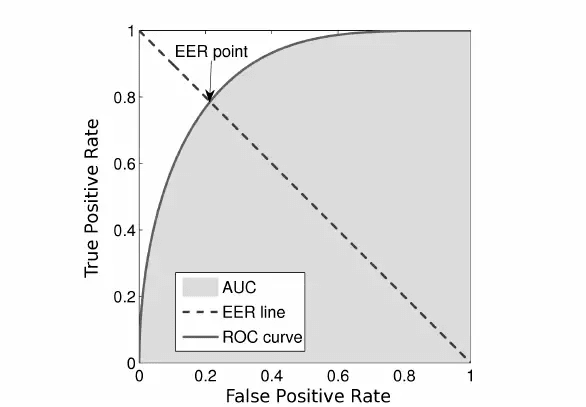
\includegraphics[width=0.9\linewidth]{EER_ROC.png}
        \caption{Связь между EER и ROC curve}
        \label{sec:Overview:Metrics:fig:EER_ROC}
    \end{figure}


    \subsection{Построение признакового пространства}
    \label{sec:Overview:Features}

    \par Различные подходы к сбору экспериментальных данных в литературе отличаются количество пользователей, принявших участие в исследовании, методами сбора и размерами собранных в итоге данных. Однако наиболее важным различием являются условия, в которых эти данные были собраны. Так, среда сбора данных может быть:

     \begin{itemize}
        \item \textsc{Контролируемой} \\
        Пользователь выполняет строго поставленные задачи. Например, кликает на появляющиеся на экране объекты \cite{Stokes, Borisov, Shen, Pilankar, Monaro}, работает только с текстовым форматом данных \cite{Fridman, Masri} или играет в компьютерные игры \cite{Kasprowski};
        \item \textsc{Неконтролируемой} \\
        Пользователь работает в привычной для него обстановке и выполняет повседневные для своей деятельности задачи \cite{Mondal, Mondal_2, Mondal_3, Antal, Khalifa, Tan, Chong, Chong2D}.
    \end{itemize}
    
    \par Сбор экспериментальных данных в контролируемой обстановке, с конкретно поставленной перед пользователем задачей, возможно даже, на конкретном компьютере, имеет серьезные недостатки. В этом случае пользователь будет больше сосредоточен на выполнении задачи, и его поведение не будет соответствовать его нормальному состоянию. По этой причине результаты экспериментов в контролируемой среде нельзя обобщить на реальную обстановку. Однако из-за совершенно неконтролируемого процесса сбора данных, может возникнуть проблема в различии количества данных, полученных от различных участников эксперимента.

    \par Нами было найдено два открытых набора данных, собранных в неконтролируемой среде: BALABIT, использующийся в работах \cite{Antal, Tan, Chong, Chong2D}, и TWOS -- \cite{Tan, Chong, Chong2D}. В остальных исследовательских публикациях используются собственные или недоступные наборы данных. Подробнее о структуре и происхождении полученных датасетов мы поговорим в разделе \ref{sec:Research:Data:Description}.

    \par Наиболее часто используемые в статьях признаки, характеризующие особенности траектории движения мыши являются:

    \begin{enumerate}
        \item кинематические характеристики:
        \begin{enumerate}
            \item перемещение, длина траектории, скорость, ускорение;
        \end{enumerate}
        \item направление движения;
        \item кривизна кривой перемещения.
    \end{enumerate}
    \vspace{10mm}

    \par Авторы \cite{Mondal} предлагают использовать особенности траектории движения компьютерной мыши, приведенные в таблице~\ref{sec:Overview:Features:table:FeaturesFormulas}, где $P_i = (x_i, y_i)$ -- координаты положения курсора. Схожие признаки используют в большинстве статьей обзора для построения признаковых пространств.

    \begin{table}[h]
        \centering
        \footnotesize
        \renewcommand{\arraystretch}{1.5}
        \renewcommand{\tabcolsep}{1mm}
        \caption{Исходное признаковое пространство}
        \begin{tabular}[c]{ || m{20mm} | c || m{20mm} | c ||}
            \hhline{|t:==:t:==:t|} 
            Признак & Формула &  Признак &  Формула \\ [2mm]
            \hhline{|:==::==:|} 
            Direction bin & \centering Divided into 8 bins (45º) &
            Curve acceleration & {\centering $\dfrac{Curvespeed}{\Delta t}$} \\
            \hhline{||-|-||-|-||}
            Actual distance & {\centering $\sqrt{(x_n-x_0)^2 + (y_n-y_0)^2}$} &
            Mean movement offset & \begin{equation*} \dfrac{1}{n} \sum_{i=1}^{n} \begin{vmatrix} P_n - P_0 \\ P_i - P_0  \end{vmatrix} / norm(P_n - P_0) \end{equation*} \\
            \hhline{||-|-||-|-||}
            Actual distance bin & {\centering Divided into 20 bins} &
            Mean movement error & {\centering \begin{equation*} \dfrac{1}{n} \sum_{i=1}^{n} \left| \begin{vmatrix} P_n - P_0 \\ P_i - P_0  \end{vmatrix} / norm(P_n - P_0) \right| \end{equation*}} \\
            \hhline{||-|-||-|-||}
            Curve length & {\centering $\dfrac{1}{n} \sum_{i=1}^{n-1} \sqrt{(x_i-x_{i+1})^2 + (y_i-y_{i+1})^2}$} &
            Mean movement variability & {\centering $\sqrt{\sum_{i=1}^{n} \dfrac{(y_i - movementoffset)^2}{n-2}}$} \\
            \hhline{||-|-||-|-||}
            Curve length bin & {\centering Divided into 20 bins} &
            Mean curvature & {\centering $\dfrac{1}{n} \sum_{i=0}^{n} \dfrac{\angle P(x_i, y_i)P(0,0)P(x_i, 0)}{\sqrt{x_{i}^2 + y_{i}^2}}$} \\
            \hhline{||-|-||-|-||}
            Length ration & {\centering $\dfrac{Curvelength}{Actualdistance}$} &
            Mean curvature change ratio & {\centering $\dfrac{1}{n} \sum_{i=0}^{n} \dfrac{\angle P(x_i, y_i)P(0,0)P(x_i, 0)}{\sqrt{(x_n-x_i)^2 + (y_n-y_i)^2}}$} \\
            \hhline{||-|-||-|-||}
            Actual speed & {\centering $\dfrac{Actualdistance}{\Delta t}$} &
            Mean curvature velocity & {\centering $\dfrac{Meancurvature}{\Delta t}$} \\
            \hhline{||-|-||-|-||}
            Curve speed & {\centering $\dfrac{1}{n} \sum_{i=0}^{n-1} \dfrac{\sqrt{(x_i-x_{i+1})^2 + (y_i-y_{i+1})^2}}{t_{i+1} - t_i}$} &
            Mean angular velocity & {\centering $\dfrac{1}{n} \sum_{i=0}^{n-2} \dfrac{\angle P_i P_{i+1} P_{i+2}}{t_{i+2} - t_i}$} \\
            \hhline{|b:==:b:==:b|} 
        \end{tabular}
        \label{sec:Overview:Features:table:FeaturesFormulas}
    \end{table}

    \par Также был рассмотрен еще ряд признаков из публикации \cite{ArsFeature}, описанных в таблице~\ref{sec:Overview:Features:table:ArsFeaturesFormulas}, где $S_{n-1}$ -- длина траектории (см. curve length в таблице~\ref{sec:Overview:Features:table:FeaturesFormulas}).

    \begin{table}[h]
        \centering
        \renewcommand{\arraystretch}{1.5}
        \renewcommand{\tabcolsep}{2mm}
        \caption{Расширение признакового пространства}
        \begin{tabular}{ || m{60mm} | c ||}
            \hhline{|t:==:t|} 
            Признак & Формула \\ [2mm]
            \hhline{|:==:|}
            minimum, maximum, mean, standard deviation and (maximum - minimum) & $x, y, v_x, v_y, v, \dot{v}, \ddot{v}$ \\
            \hhline{||-|-||}
            Траектория центра масс (TCM: Trajectory Center of Mass) & $ \dfrac{1}{S_{n-1}} \sum_{i=1}^{n-1} t_{i+1} \sqrt{(x_{i+1} - x_{i})^2 + (y_{i+1} - y_i)^2} $ \\
            \hhline{||-|-||}
            Коэффициент рассеивания (SC: Scattering Coefficient) &  $ \dfrac{1}{S_{n-1}} \sum_{i=1}^{n-1} t_{i+1}^2 \sqrt{(x_{i+1} - x_{i})^2 + (y_{i+1} - y_i)^2} - TCM^2 $ \\
            \hhline{||-|-||}
            Третий момент ($M_3$) & $ \dfrac{1}{S_{n-1}} \sum_{i=1}^{n-1} t_{i+1}^3 \sqrt{(x_{i+1} - x_{i})^2 + (y_{i+1} - y_i)^2} $ \\
            \hhline{||-|-||}
            Четвертый момент ($M_4$) & $ \dfrac{1}{S_{n-1}} \sum_{i=1}^{n-1} t_{i+1}^4 \sqrt{(x_{i+1} - x_{i})^2 + (y_{i+1} - y_i)^2} $ \\
            \hhline{||-|-||}
            Траектория кривой (TCrv: Trajectory Curvature) & $ \dfrac{\dot{x}\ddot{y} - \ddot{x}\dot{y}}{(\dot{x}^2 + \dot{y}^2)^\tfrac{3}{2}} $ \\
            \hhline{||-|-||}
            Кривизна скорости (VCrv: Velocity Curvature) & $ \dfrac{\ddot{v}}{(1 + \dot{v}^2)^\tfrac{3}{2}} $ \\
            \hhline{|b:==:b|}
        \end{tabular}
        \label{sec:Overview:Features:table:ArsFeaturesFormulas}
    \end{table}

    \par Получающиеся в итоге признаковые пространства имеют небольшую размерность и поэтому в качестве метода их предобработки зачастую используют только нормализацию \cite{Fridman, Kasprowski, Tan}, заданную формулой~\ref{sec:PracticalPart:formula:StandartScaler}, и предварительную отчистку от выбросов \cite{Tan, Pilankar}.
    \begin{equation}
    \label{sec:PracticalPart:formula:StandartScaler}
        \hat{x}  = \frac{x - \mathsf{E} x}{\sqrt{\Variance x}}
    \end{equation}
    \noindent где $\mathsf{E} x$ -- математическое ождание наблюдения, а $\Variance x$ -- его дисперсия. 


    \subsection{Построение модели пользователя}
    \label{sec:Overview:Model}

    В работах \cite{Mondal_2, Shen} проводится сравнение качества работы существующих методов аутентификации на основе анализа работы пользователя с компьютерной мышью. Дополняя их результатами исследований последних лет, мы сформировали сводную таблицу~\ref{sec:Overview:Model:table:Result} с методами, демонстрируюющими наилучшие показатели. Основными лидерами являются:

    \begin{itemize}
        \item \textsc{OneClassSVM} \\
        Благодаря kernel trick, модель способна проводить нелинейные разделяющие границы. Затачивается на обучающей выборки и поэтому отлично подходит для решения задачи поиска аномалий.
        \item \textsc{Sparse autoencoder} \\
        Автокодировщик с ограничением разреженности на нейроны скрытого слоя за счет использования L1-, L2-регуляризации. Обнаруживает структурных закономерностей в данных на скрытых слоях.
    \end{itemize}

    \begin{table}[h]
        \centering
        \renewcommand{\arraystretch}{1.5}
        \renewcommand{\tabcolsep}{2mm}
        \caption{Качество работы методов из обзора}
        \begin{tabular}{ || l | c ||}
            \hhline{|t:==:t|} 
            Метод                              & EER, \% \\ [2mm]
            \hhline{|:==:|}
            k Nearest Neighbor (kNN)           & 2.6  \\ \hline
            Gaussian Naive Bayers              & 8.0  \\ \hline
            Decision Tree (DT)                 & 7.5  \\ \hline
            Logistic Model Tree (LMT)          & 5.0  \\ \hline
            \textbf{OneClassSVM (OC-SVM)}      & 1.37 \\ \hline
            Hopfield network model             & 4.5  \\ \hline
            \textbf{Sparse autoencoder (SAE)}  & 1.5  \\ \hline
            restricted Boltzmann machine (RBM) & 2.8  \\
            \hhline{|b:==:b|}
        \end{tabular}
        \label{sec:Overview:Model:table:Result}
    \end{table}

    Рассмотрим подробнее методы решения поставленной задачи в разделе~\ref{sec:Research:Model}.


    \subsection{Выводы}
    \label{sec:Overview:Conclusions}

    По результатам обзора:
    \begin{enumerate}
        \item Рассмотрены существующие решения и качество их работы. Основным недостатков многих работ является постановка перед участниками эксперимента конкретной задачи. Мы же хотим обеспечивать защиту пользователей в произвольной и привычной для них среде. Также проблемой для многих систем стало падение качества аутентификации после смены набора данных.
        \item Были рассмотрены признаки, характеризующие траекторию движения компьютерной мыши, которые составят признаковое пространтво для обучения моделей.
        \item Были найдены наборы данных для проведения собственных экспериментальных исследований. Их структура будет подробно описана в разделе~\ref{sec:Research:Data:Description}.
        \item Лучший результат демонстрирует одноклассовый метод опорных векторов. Поэтому в дальнейшем мы сфокусируемся на рассмотрении классических методов машинного обучения для решения поставленной задачи. А затем рассмотрим методы, основанные на использовании нейронных сетей.
    \end{enumerate}

    \newpage



    \section{Исследование и построение решения задачи}
    \label{sec:Research}

    \subsection{Сбор данных и извлечение признаков}
    \label{sec:Research:Data}

    \subsubsection{Описание наборов данных}
    \label{sec:Research:Data:Description}

    \par Как было сказано в обзоре, для расширения области применения и возможностей нашей системы необходимо для обучения использовать данные, собранные в неконтролируемой среде.

    \par По итогам обзора было выявлено 3 набора данных для оценки производительности поведенческих биометрических алгоритмов на основе динамики работы с компьютерной мышью в целях аутентификации пользователя.

    \begin{itemize}
        \item \textsc{BALABIT} \cite{BALABIT} \\
        Это датасет, предоставленный компанией BalaBit IT Security, специализирующейся на разработке программного обеспечения и сервисов для информационной безопасности, в 2016 году в рамках одноименного конкурса Balabit Mouse Dynamics Challenge. Набор данных доступен для исследователей и экспертов в области IT-безопасности и науки, используется в большинстве научных статей обзора. Данные собраны в неконтролируемой среде и включают информацию о времени и позиционировании указателя компьютерной мыши. В эксперименте приняло участие 10 человек. В среднем для обучения мы имеем 43 $\pm$ 17 часов работы на каждого пользователя.

        \item \textsc{TWOS} (The Wolf Of SUTD) \cite{TWOS} \\
        Этот датасет был предоставлен во время конкурса , организованного Сингапурским университетом технологии и дизайна в марте 2017 года. Набор данных содержит действия 24 пользователей, которые собирались в неконтролируемой среде в течение 5 дней. Однако информация о взаимодействии с компьютерной мышью есть только для 4 пользователей. В среднем мы имеем 10 $\pm$ 1 час работы на каждого пользователя.

        \item \textsc{DATAIIT} \\
        Датасет, собранный на нашей кафедре в рамках исследования задачи динамической аутентификации пользователя в 2015 году. Данные собраны в неконтролируемой среде. В эксперименте приняло участие 20 человек. В среднем мы имеем 21 $\pm$ 5 часов работы на каждого пользователя.
    \end{itemize}


    \subsubsection{Структура данных}
    \label{sec:Research:Data:Struct}
    
    \par Набор данных был разбит на тренировочную и тестовую части, 75\% и 25\% от исходных данных соответвенно. Каждая часть содержит в себе записи об авторизированных сеансах всех пользователей из множества $\mathfrak{U}=\{U_1, \ldots, U_j, \ldots, U_q\}$. Работа пользователя разбита на сессии разной продолжительности $U_j = \{S_1, \ldots, S_i, \ldots, S_m\}$, где каждая сессия $S_i \in U_j$ $(i = \overline{1,m}, \; j = \overline{1,q})$ содержит записи вида $(time, xpos, ypos)$. Далее каждую сессию мы разбиваем на сегменты с ограничением по временному порогу сверху (назовем эту операцию T-Time Split) и по минимальному количеству действий в этот промежуток времени снизу. По полученному сегменту строится один вектор признаков.

    \par Графическая визуализация структуры данных представлена на рисунке~\ref{sec:Research:Data:Description:fig:DataStructure}

    \vspace{10mm}
    \begin{figure}[h!]
        \centering
        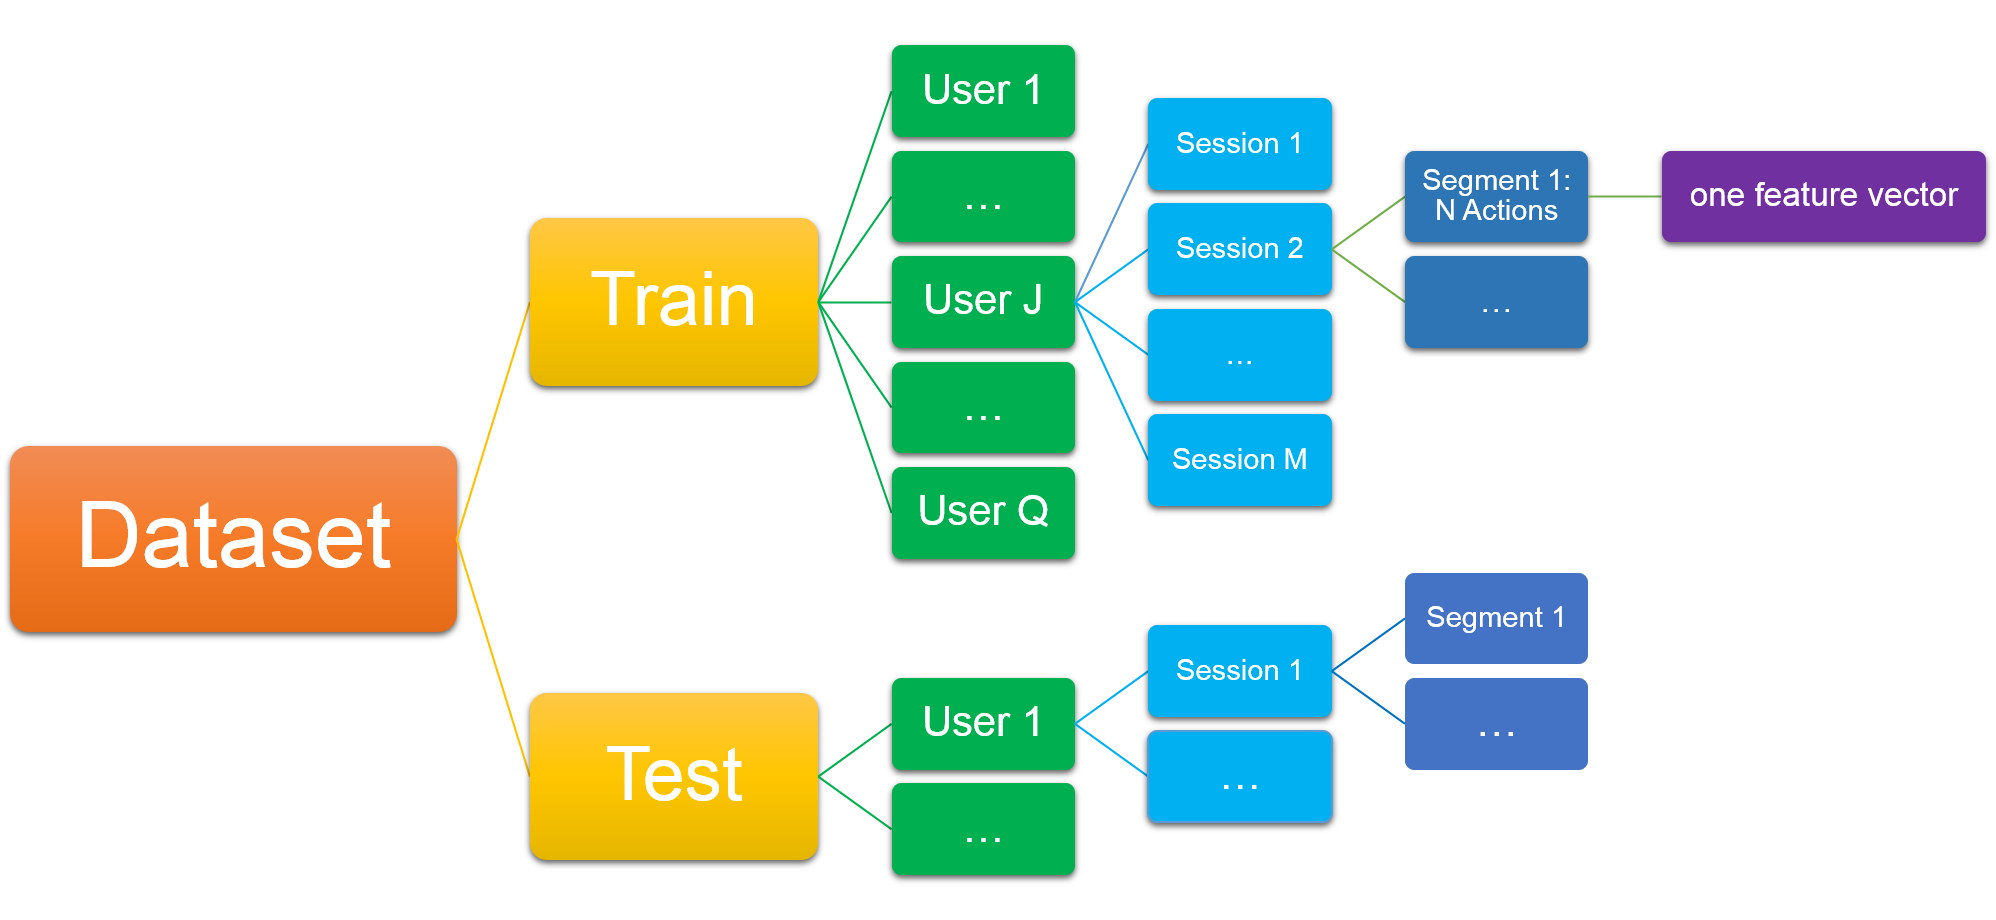
\includegraphics[width=\linewidth]{DataStructure.png}
        \caption{Структура данных}
        \label{sec:Research:Data:Description:fig:DataStructure}
    \end{figure}
    \vspace{5mm}


    \subsubsection{Выявленные особенности данных}
    \label{sec:Research:Data:Features}

    \par Во время анализа данных были обнаружены следующие особенности:

    \begin{enumerate}
        \item полностью дублирующиеся записи в таблице;
        \item дубликаты временных меток;
        \item множественные дубликаты положения мыши (зацикливание);
        \item сверхбольшие значения координат;
        \item в наборе данных BALABIT:
        \begin{enumerate}
            \item в состоянии прокрутки колеса (Scroll) положение мыши перемещается в начало координат;
            \item основная работа пользователей происходит в левом нижнем углу экрана.
        \end{enumerate}
    \end{enumerate}

    \noindent Все особенности были устранены из наборов данных.


    \subsection{Построение признакового пространства}
    \label{sec:Research:FeatureSpace}

    \par Так как 16 признаков, объявленных в таблице~\ref{sec:Overview:Features:table:FeaturesFormulas} может оказаться недостаточно для уникальности отдельно взятого вектора признаков, мы сформируем признаковое пространство, как конкатенацию признаков из таблицы \ref{sec:Overview:Features:table:FeaturesFormulas} и \ref{sec:Overview:Features:table:ArsFeaturesFormulas}. Получившееся признаковое пространство имеет размерность 78 признаков на вектор.

    \par Для обработки признакового пространство нами было предложено использовать следующие методы:

    \subsubsection{Квантование}
    \label{sec:Research:FeatureSpace:Quantile}

    \par Квантование \cite{BINNING} -- процесс предобработки данных, при котором непрерывные данные преобразуются в дискретные путем замены значений интервалами, каждый из которых представляет некоторый диапазон. Различают два основных метода квантования:

    \begin{enumerate}
        \item \textsc{Интервальный} \\
        Диапазон изменения значений признака разделяется на равные интервалы. Данный метод используется, если значения равномерно распределены на всей области значений, т.е. в результате квантования не будет интервалов, в которых значения почти отсутствуют или, наоборот, плотных интервалов.
        \item \textsc{Квантильный} \\
        Ширину интервалов выбирают таким образом, чтобы в каждый из них попало примерно одинаковое количество значений.
    \end{enumerate}

    \par Согласно \cite{Kazachuk}, одним из наиболее популярных методов предобработки признаков, используемых для мультимодальных распределений, является именно квантильная дискретизация. Этот подход ранее не применялся к анализу данных работы с компьютерной мышью.

    \par На рисунке~\ref{sec:Research:FeatureSpace:Quantile:fig:Quantile} продемонстрировано разбиение данных на 4 квантиля (т.н. квартили).

    \begin{figure}[h!]
        \centering
        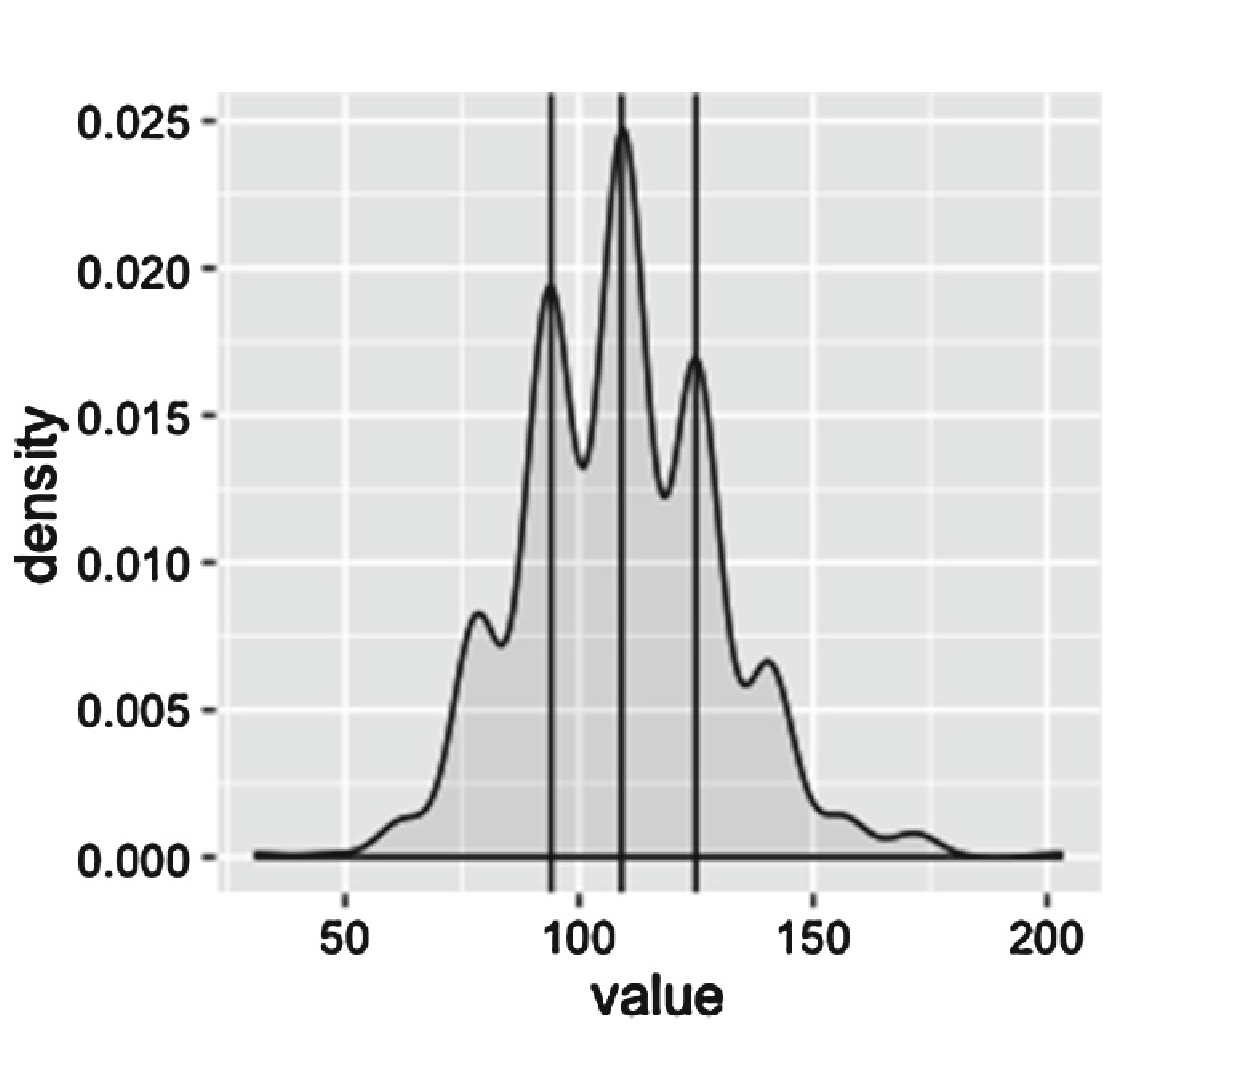
\includegraphics[width=0.75\linewidth]{quantile.png}
        \caption{Квантильная дискретизация данных}
        \label{sec:Research:FeatureSpace:Quantile:fig:Quantile}
    \end{figure}


    \subsubsection{One-Hot Encoding}
    \label{sec:Research:FeatureSpace:OneHotEncoding}

    \par One-Hot Encoding -- это кодировка, с помощью которой категориальные признаки преобразуются в дискретную форму, для лучшего качества прогнозирования методами машинного обучения. Под категориальным признаком подразумевается признак, значения которого обозначают принадлежность объекта к какой-то категории. Например, город со значением из множества \{Москва, Анапа, Сургут, \ldots\}.

    \par Пусть $ \mathfrak{V} = \{V_1, \ldots, V_i, \ldots, V_s\} $ -- множество уникальных значений категориального признака $V$. Тогда каждое $V_i \in \mathfrak{V}$ $(i = \overline{1,s})$ преобразуется в $s$ новых признаков, где $i$-й признак будет принимать значение 1, а все остальные -- 0.

    \par Даннный подход устраняет проблему иерархии (порядка), возникающую при вещественной кодировке категориальных признаков, когда $V_i \mapsto i \in \mathbb{N}(\mathbb{R})$.

    \par Однако данный метод также имеет недостаток, заключающийся в добавлении большего количества признаков в набор данных. Это может привести к значительному увеличению признакового пространства, если категориальный признак будет иметь много уникальных значений.




    \subsubsection{Градиентный бустинг}
    \label{sec:Research:FeatureSpace:GradientBoostingClassifier}

    \par Преимущество использования ансамблей деревьев решений, таких как градиентный бустинг \cite{GBM}, заключается в том, что они могут предоставлять оценку важности призаков из обученной модели.

    \par Как правило, важность обеспечивает оценку, которая указывает, насколько полезным был каждый признак при построении деревьев решений в модели. Чем больше атрибут используется для принятия ключевых решений с деревьями решений, тем выше его относительная важность.

    \par Важность рассчитывается для отдельного дерева решений, затем значения характеристик усредняются по всем деревьям решений в модели.


    \subsection{Построение модели пользователя}
    \label{sec:Research:Model}

    \subsubsection{Задача поиска аномалий}
    \label{sec:Research:Model:Anomaly}

    \par Согласно \cite{Dyakonov, NoveltyDetection}, в анализе данных есть два направления, которые занимаются поиском аномалий: детектирование выбросов (Outlier Detection) и детектирование новизны (Novelty Detection). Как и выброс, новый объект — это объект, который отличается по своим свойствам от объектов обучающей выборки. Но в отличие от выброса, его в самой выборке пока нет. Задачей обнаружения новизны является идентификация новых или неизвестных данных, о которых система не знает во время обучения. Это означает, что задача поиска аномалий относится к классу unsupervised learning, т.е является задачей обучения без учителя.

    \par Например, при анализе замеров температуры и отбрасывании аномально больших или маленьких значений, происходит борьба с выбросами. А при создании алгоритма, который для каждого нового замера оценивает, насколько он похож на предыдущие, и выбрасывает аномальные — детектирование новизны.

    \par Областей, где возникает задача поиска аномалий, достаточно много:

    \begin{enumerate}
        \item обнаружение вторжений;
        \item обнаружение подозрительных банковских операций;
        \item обнаружение неполадок в механизмах;
        \item обнаружение инсайдров на бирже;
        % \item обнаружение мошенничества
        \item медицинская диагностика;
        \item сейсмология;
    \end{enumerate}

    \par Особенности этой задачи заключаются в том, что присутсвует явный дисбаланс классов (аномалии достаточно редки), а также в том, что тренировочные данные уже могут содержать аномальные наблюдения, о которых мы можем не знать. Такие наблюдения нужно идентифицировать и удалить из тренировочных данных на этапе предобработки признаков, чтобы система не приняла аномальные наблюдения за нормальные.

    \par Стоит отметить, что, в общем случае, мы не можем свести задачу поиска аномалии к бинарной классификации, т.к. в реальной жизни у нас может не оказаться размеченных аномальных наблюдений для обучения.

    \par В следующих разделах мы рассмотрим классические методы машинного обучения для решения задачи поиска аномалий.


    \subsubsection{One Class SVM}
    \label{sec:Research:Model:OneClassSVM}

    \par Метод опорных векторов (SVM: Support Vector Machine) \cite{SVM} -- это семейство мощного статистического обучения методов классификации и регрессии. Они доказали свою эффективность во многих практических применениях. SVM основывается на индуктивном принципе минимизации структурных рисков (SRM: Structural Risk Minimization).

    \par Одноклассовый метод опорных векторов (OC-SVM: One Class SVM) \cite{OC-SVM} был предложен, как расширение SVM, для выявления новизны или выбросов в наборах данных. Важную роль OC-SVM играет в области обнаружения вторжений.

    \par Основная идея алгоритма заключается в поиске геперплоскости в признаковом пространстве, которая максимально отдаляет данные от начала координат.

    \begin{figure}[h!]
        \centering
        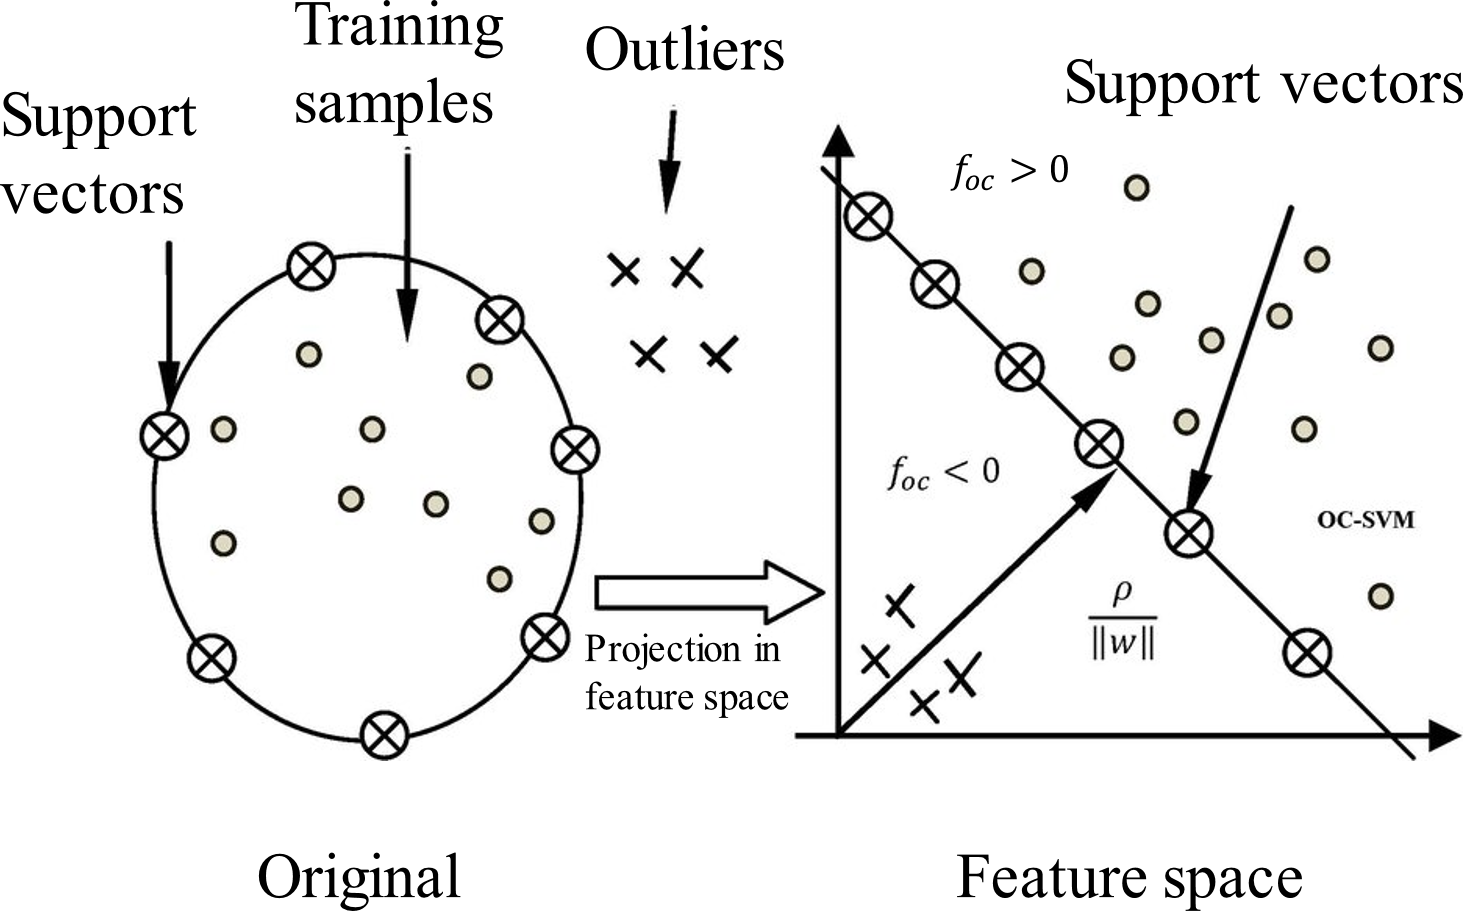
\includegraphics[width=0.8\linewidth]{OneClassSVM.png}
        \caption{One Class SVM: принцип работы}
        \label{sec:Research:Model:OneClassSVM:fig:OneClassSVM}
    \end{figure}


    \subsubsection{Isolation Forest}
    \label{sec:Research:Model:IsolationForest}

    \par Изоляционный лес (IF: Isolation Forest) \cite{IsolationForest}, как и любой другой метод ансамбля деревьев, построен на основе деревьев решений (DT: Decision Tree). Алгоритм обучения строит ансамбль изоляционных деревьев на основе рекурсивной и рандомизированной процедуры структурированного разбиения: сначала случайным образом выбирается объект, а затем выбирается случайное значение между минимальным и максимальным значением выбранного объекта.

    \par Выбросов в данных не много и, зачастую, они находятся дальше от обычных наблюдений в пространстве признаков. Вот почему при использовании такого случайного разбиения они должны быть идентифицированы ближе к корню дерева. В случае аномальных наблюдений необходимо меньше расщеплений.

    \begin{figure}[h!]
        \centering
        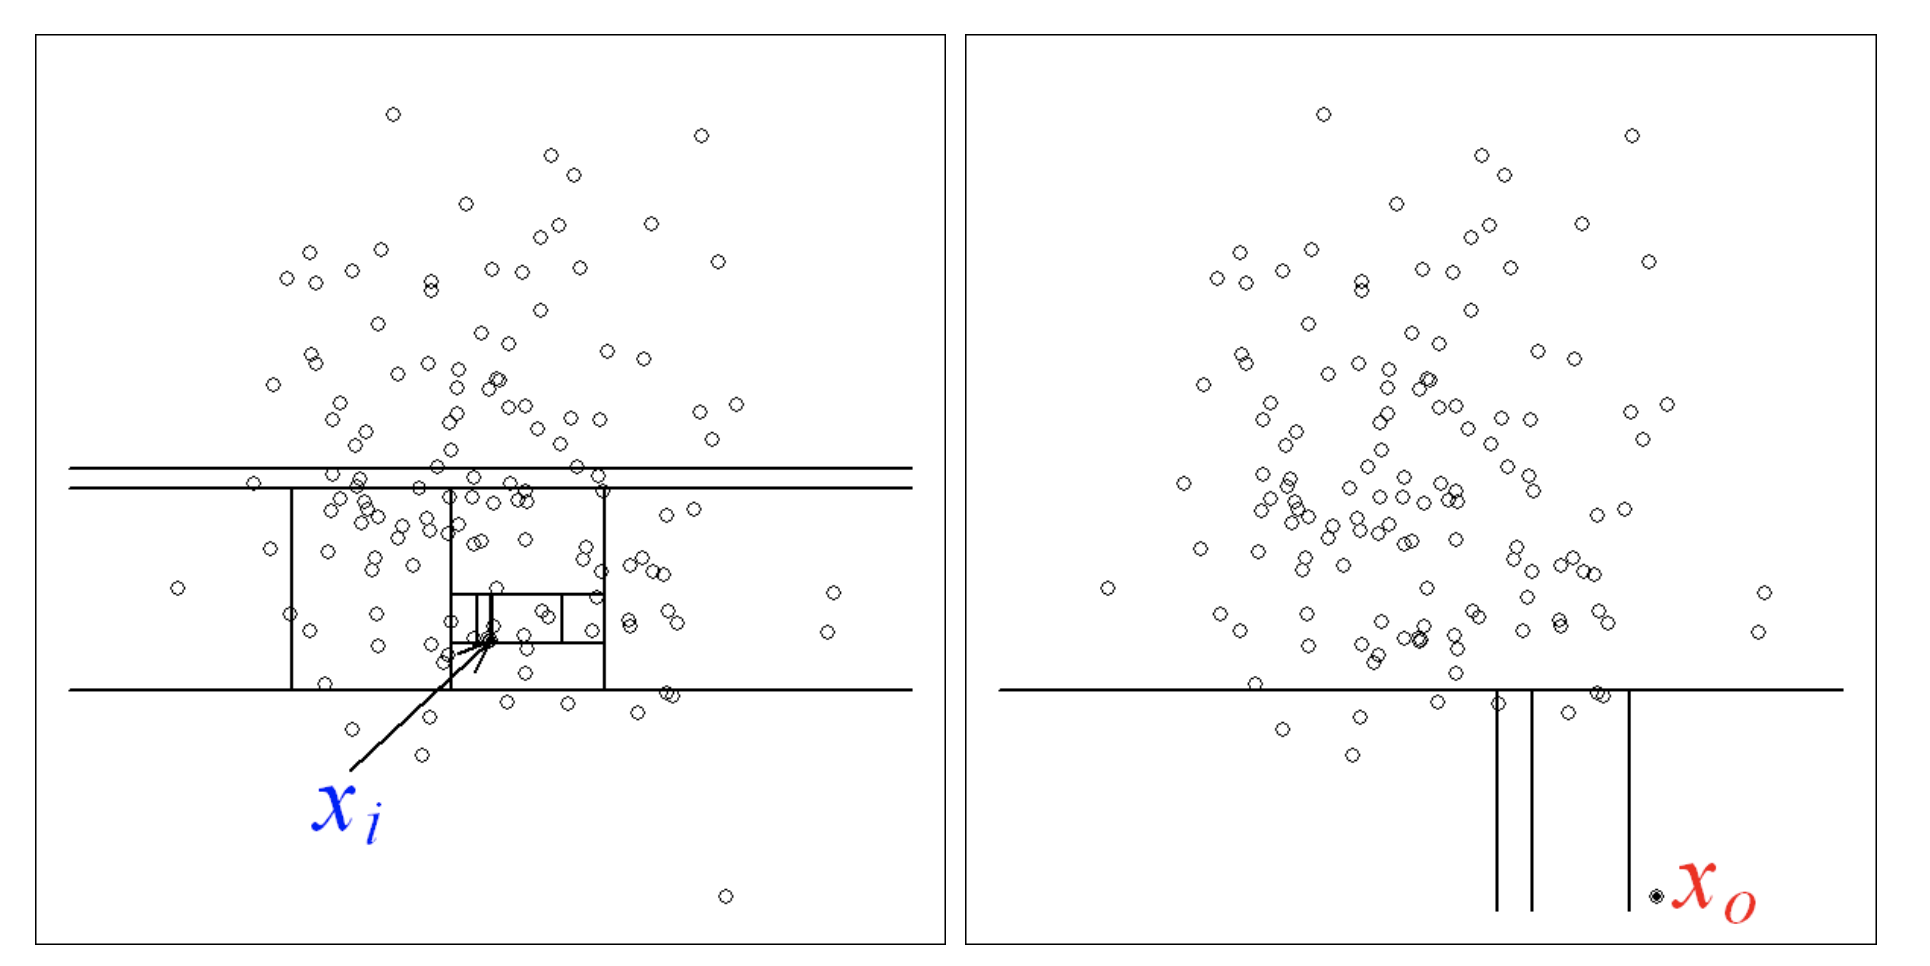
\includegraphics[width=0.8\linewidth]{IsolationForest.png}
        \caption{Isolation Forest: Определение нормальных и аномальных наблюдений}
        \label{sec:Research:Model:IsolationForest:fig:IsolationForest}
    \end{figure}

    \par Так, на рисунке~\ref{sec:Research:Model:IsolationForest:fig:IsolationForest} синим цветом показано нормальное наблюдение $x_i$, а красным -- аномальное $x_0$. Здесь аномальная точка была разделена в несколько шагов, в то время как для изоляции нормального наблюдения потребовалось больше разделений.

    \par Для принятия решения об аномальности наблюдения алгоритм используют следующую функцию:
    \begin{equation}
    \label{sec:Research:Model:IsolationForest:formula:IF}
        S(x,n) = 2^{-\frac{\mathsf{E}(h(x))}{c(n)}}
    \end{equation}

    \noindent где $\mathsf{E}(h(x))$ -- средняя длина пути наблюдения $x$ , $c(n)$ -- средняя длина пути неудачного поиска в бинарном дереве поиска, а $n$ -- количество внешних узлов.

    \par Каждое наблюдение получает индекс аномальности, на основе которого принимается решение:
    \begin{itemize}
        \item Оценка, близкая к 1, указывает на аномальность наблюдения;
        \item Оценка, близкая к 0, указывает на нормальное поведение наблюдения.
    \end{itemize}


    \subsubsection{Local Outlier Factor}
    \label{sec:Research:Model:LocalOutlierFactor}

    \par Локальный уровень выброса (LOF: Local Outlier Factor) \cite{LOF} обнаруживает выбросы на основе локальной плотности точек, которые являются выбросами по отношению к их локальной окрестности, а не по отношению к глобальному распределению данных. Чем выше значение LOF для наблюдения, тем более аномальным оно является. Точка считается аномальной, если ее локальная плотность значительно отличается от плотности соседних точек. LOF в точке P определяется как:
    \begin{equation}
    \label{sec:Research:Model:LocalOutlierFactor:formula:LOF}
        LOF(P) = \sum \text{(расстояние до соседей)} \cdot \sum \text{(локальная плотность соседей)}
    \end{equation}

    \noindent Таким образом, LOF в точке P может принимать:

    \begin{itemize}
        \item большое значение, если точка P находится далеко от своих соседей и его соседи имеют высокую локальную плотность (т.е. они близки к своим соседям): \\ 
        $ LOF(P) = \sum {\text{(большое расстояние)}} \cdot \sum \text{(большая плотность)} = \text{большое значение}$
        \item среднее значение, если P находится далеко от своих соседей и его соседи имеют малую локальную плотность: \\
        $ LOF(P) = \sum \text{(большое расстояние)} \cdot \sum \text{(маленькая плотность)} = \text{среднее значение} $
        \item маленькое значение, если P находится близко к своим соседям и его соседи имеют малую локальную плотность: \\
        $ LOF(P) = \sum \text{(маленькое расстояние)} \cdot \sum \text{(маленькая плотность)} = \text{маленькое значение} $
    \end{itemize}

    \begin{figure}[h!]
        \centering
        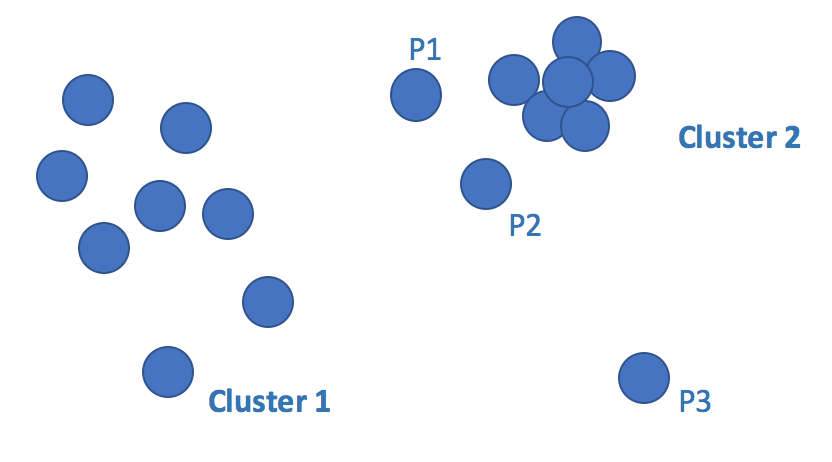
\includegraphics[width=0.6\linewidth]{LocalOutlierFactor.png}
        \caption{Local Outlier Factor: Определение нормальных и аномальных наблюдений}
        \label{sec:Research:Model:LocalOutlierFactor:fig:LocalOutlierFactor}
    \end{figure}

    \par Так в приведенном пространстве признаков на рисунке~\ref{sec:Research:Model:LocalOutlierFactor:fig:LocalOutlierFactor} метод LOF, кроме очевидного аномального наблюдения P3, определит точки P1 и P2 как выбросы, которые являются локальными для второго кластера.


    \subsubsection{Elliptic Envelope}
    \label{sec:Research:Model:EllipticEnvelope}

    \par Эллипсоидальная аппроксимация данных (EE: Elliptic Envelope) \cite{EE} -- ковариационная оценка, предполагающая, что данные имеют распределение Гаусса. Ограничивающий контур имеют эллиптическую форму.

    \par Процедура EE использует алгоритм FAST-Minimum Covariance Determinate для оценки размера и формы эллипса. Данный алгоритм выбирает неперекрывающиеся подвыборки данных и вычисляет среднее значение $\mu$ и ковариационную матрицу $C$ в признаковом пространстве для каждой подвыборки. Расстояние Махаланобиса $dMH$ вычисляется для каждого многомерного вектора данных (признака) $x$ в каждой подвыборке, по формуле:
    \begin{equation}
    \label{sec:Research:Model:EllipticEnvelope:formula:MahalanobisDistance}
        dMH = \sqrt{(x-\mu)^T C (x-\mu)}
    \end{equation}

    \noindent Затем данные упорядочивают по возрастанию значений $dMH$. Эта процедура повторяется до сходимости определителя матрицы ковариации. Ковариационная матрица с наименьшим определителем из всех подвыборок образует эллипс, который охватывает часть исходных данных. Данные в пределах поверхность эллипса считаются нормальными, а вне эллипса -- аномальными.


    \subsubsection{Визуализация работы методов}
    \label{sec:Research:Model:Visualization}

    \par В данном разделе мы визуализируем работу описанных ранее методов, определим достоинства и недостатки каждого с целью выявления наилучшего кандидата для решения поставленной задачи.

    \par Для этого сформируем двумерный набор тестовых данных (toy dataset), содержащий 100 объектов, 5\% которых будут выбросами. Первый набор данных (a) состоит из одного кластера, второй (b) -- из трех, а последний набор (c) -- из десяти, что позволит сильнее разнести объекты в пространстве признаков. Синим цветом помечены нормальные наблюдения, красным -- аномальные (выбросы). Алгоритмы машинного обучения взяты из бесплатной библиотеки машинного обучения для языка программирования Python -- scikit-learn.

    % features
    \begin{figure}[h!]
        \centering
        \subfigure[]{
            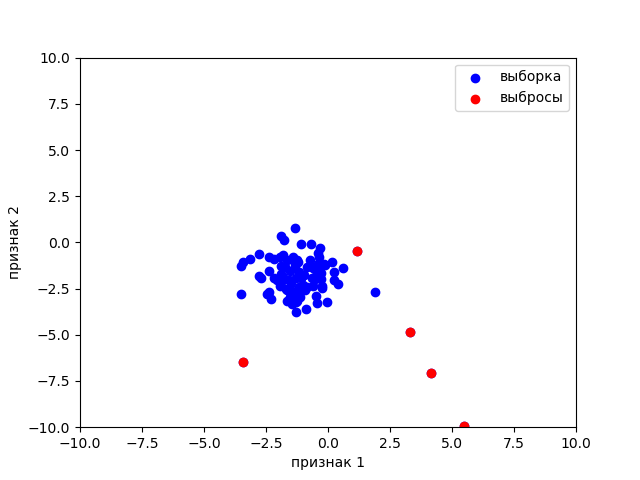
\includegraphics[width=0.29\linewidth]{features_1.png}
            \label{sec:Research:Model:Visualization:fig:featueres:1}
        }
        \subfigure[]{
            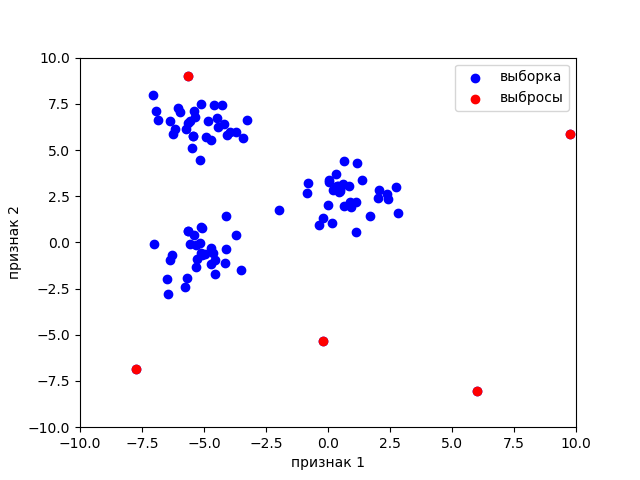
\includegraphics[width=0.29\linewidth]{features_3.png}
            \label{sec:Research:Model:Visualization:fig:featueres:3}
        }
        \subfigure[]{
            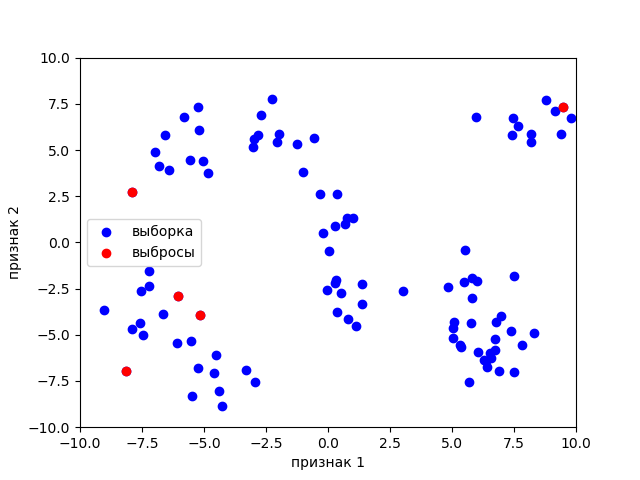
\includegraphics[width=0.29\linewidth]{features_10.png}
            \label{sec:Research:Model:Visualization:fig:featueres:10}
        }
        \caption{Тестовые наборы данных}
        \label{sec:Research:Model:Visualization:fig:featueres}
    \end{figure}

    % \noindent Условные обозначения на следующих графиках:
    % \begin{itemize}
    %     \item центр кластеров помечен более темным оттенком;
    %     \item желтая пунктирная линия -- разделяющая поверхность;
    %     \item белые точки -- нормальные наблюдения;
    %     \item красные точки -- аномальные наблюдения.
    % \end{itemize}

    \textbf{One Class SVM} \\

    \noindent \textsc{Гиперпараметры}
    \begin{itemize}
        \item kernel (ядро): радиальное (rbf). Доступны также линейное (linear), сигмоидальное (sigmoid) и полиномиальное (poly), но они покзывают низкое качество идентификации в задаче поиска аномалий:
        \item nu ($\nu$) $\in [0, 1]$ – верхняя граница на \% ошибок. В нашем случае nu=0.05.
    \end{itemize}

    \noindent \textsc{Достоинства}
    \begin{itemize}
        \item благодаря kernel trick, модель способна проводить нелинейные разделяющие границы. Идея заключается в том, что классы, линейно неразделимые в текущем признаковом пространстве, могут стать разделимыми в пространстве более высокой размерности.
    \end{itemize}

    \noindent \textsc{Недостатки}
    \begin{itemize}
        \item может очень сильно переобучиться и выдавать большое количество ложно отрицательных результатов;
        \item нужно быть абсолютно уверенным, что тренировочные данные не содержат никаких выбросов, иначе алгоритм будет считать их нормальными наблюдениями.
    \end{itemize}

    % OneClassSVM
    \begin{figure}[h!]
        \centering
        \subfigure[]{
            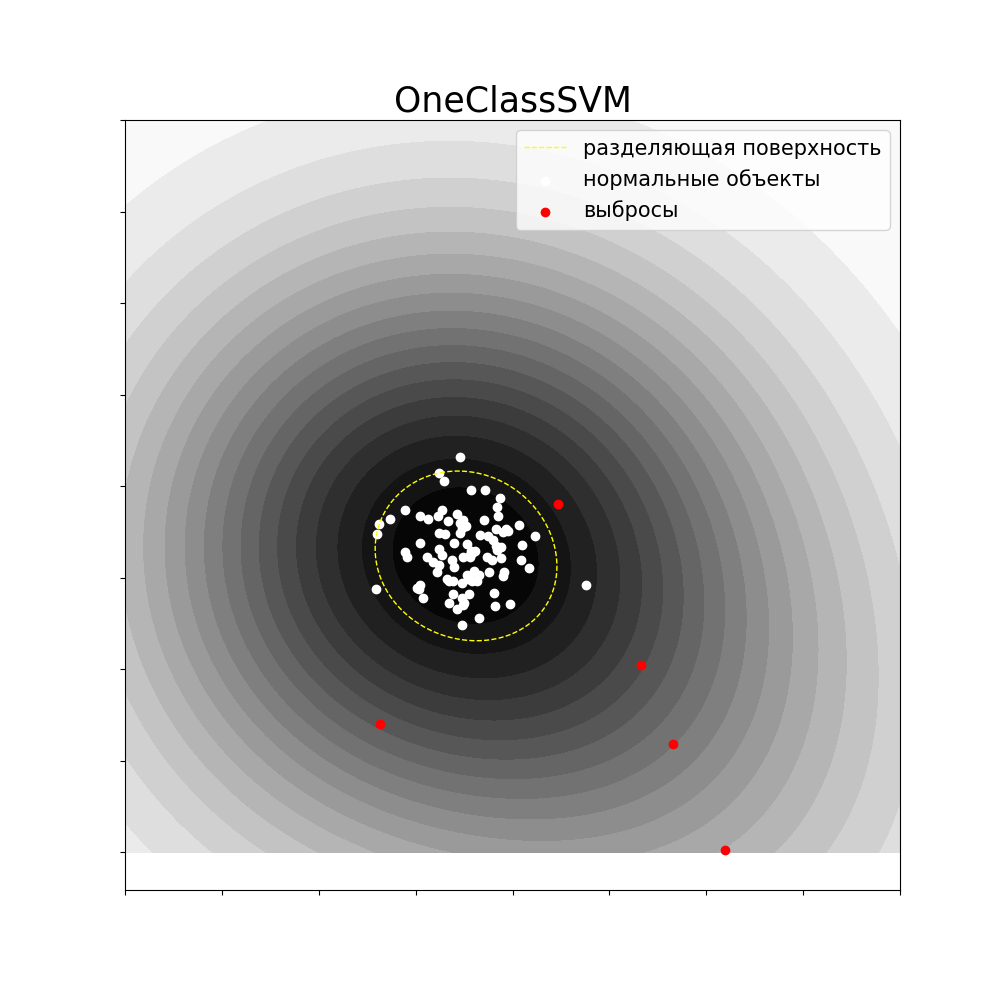
\includegraphics[width=0.3\linewidth]{OneClassSVM_1.png}
            \label{sec:Research:Model:Visualization:fig:OneClassSVM:1}
        }
        \subfigure[]{
            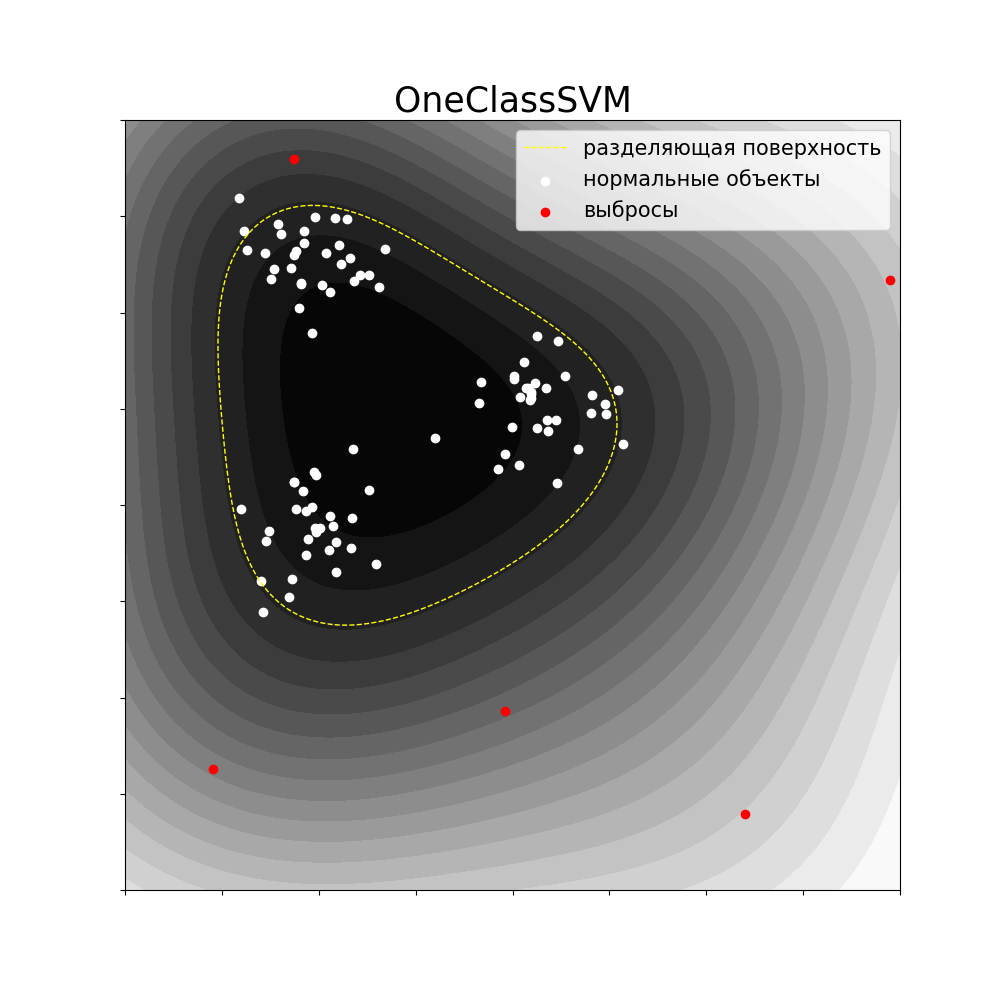
\includegraphics[width=0.3\linewidth]{OneClassSVM_3.png}
            \label{sec:Research:Model:Visualization:fig:OneClassSVM:3}
        }
        \subfigure[]{
            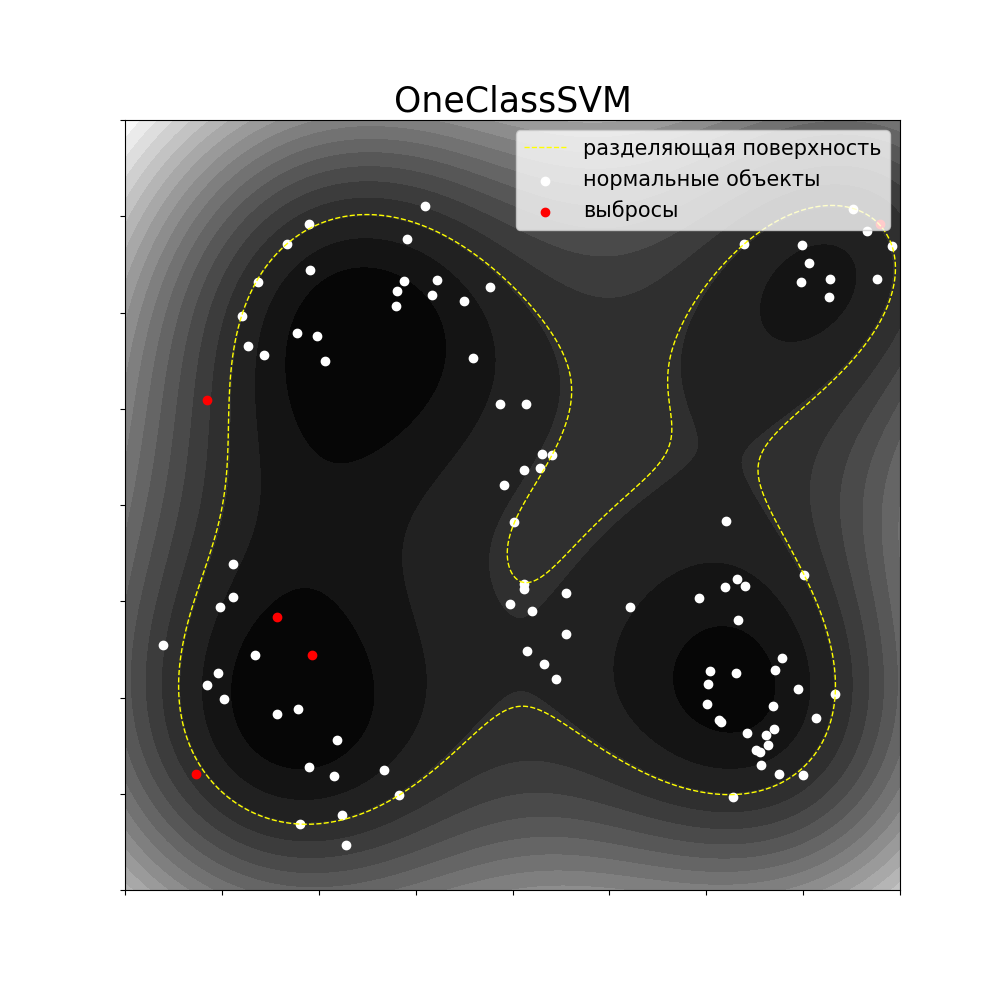
\includegraphics[width=0.3\linewidth]{OneClassSVM_10.png}
            \label{sec:Research:Model:Visualization:fig:OneClassSVM:10}
        }
        \caption{One Class SVM: визуализация работы метода на тестовых данных}
        \label{sec:Research:Model:Visualization:fig:OneClassSVM}
    \end{figure}

    \par Как видно на рисунке~\ref{sec:Research:Model:Visualization:fig:OneClassSVM} одноклассовый метод опорных векторов хорошо проводит разделяющую поверхность, охватывая большую часть тренировочных данных.

    \par Алгоритм больше подходит для детектирования новизны, т.к. затачивается под обучающую выборку и поэтому лучше подходит для решения нашей задачи.

    \newpage


    \textbf{Isolation Forest} \\

    \noindent \textsc{Гиперпараметры}
    \begin{itemize}
        \item n\_estimators – число деревьев;
        \item max\_samples – объем выборки для построения одного дерева;
        \item contamination – доля выбросов в выборке.
    \end{itemize}

    \noindent \textsc{Достоинства}
    \begin{itemize}
        \item алгоритм распознает аномалии различных видов: как изолированные точки с малой локальной плотностью, так и небольшие кластеры аномалий;
        \item эффективность: сложность алгоритма $ O(n \log n) $;
        \item устойчив к проклятию размерности.
    \end{itemize}

    \noindent \textsc{Недостатки}
    \begin{itemize}
        \item алгоритм больше подходит для поиска выбросов в данных, а не новизны.
    \end{itemize}

    % IsolationForest
    \begin{figure}[h!]
        \centering
        \subfigure[]{
            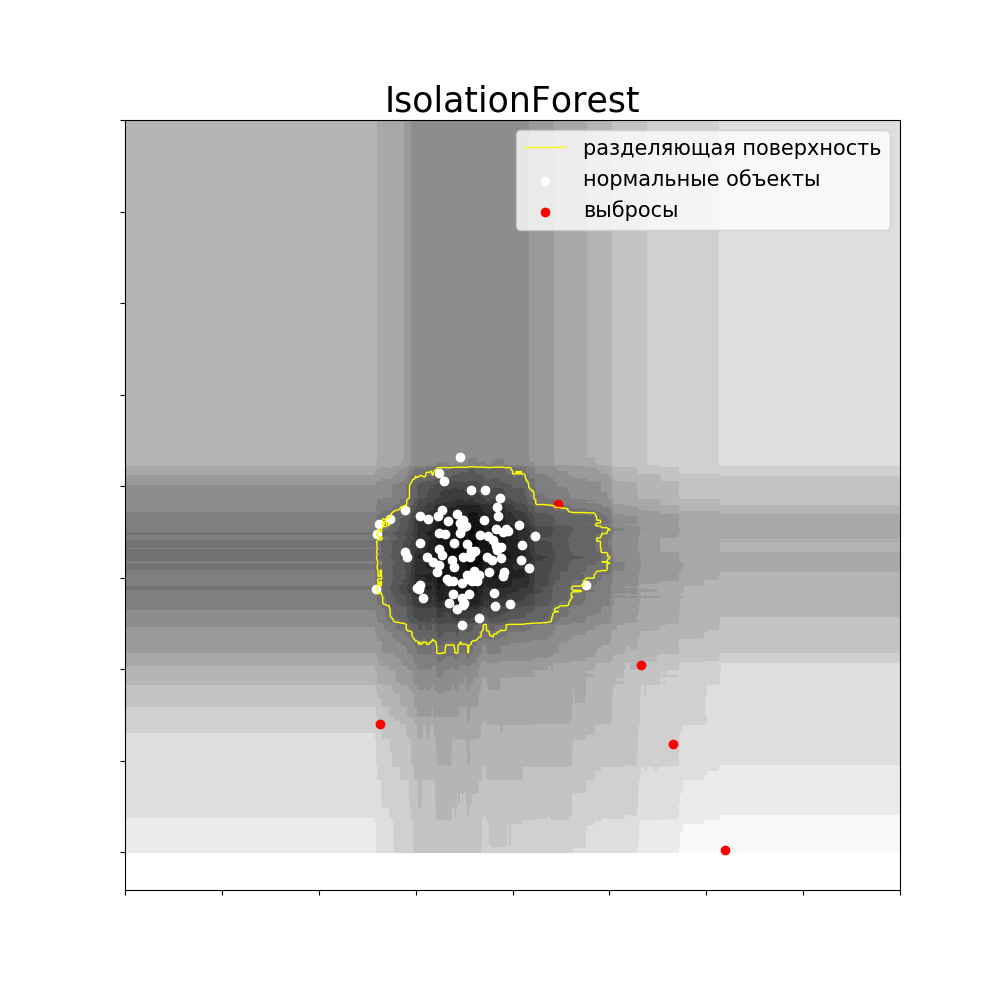
\includegraphics[width=0.3\linewidth]{IsolationForest_1.png}
            \label{sec:Research:Model:Visualization:fig:IsolationForest:1}
        }
        \subfigure[]{
            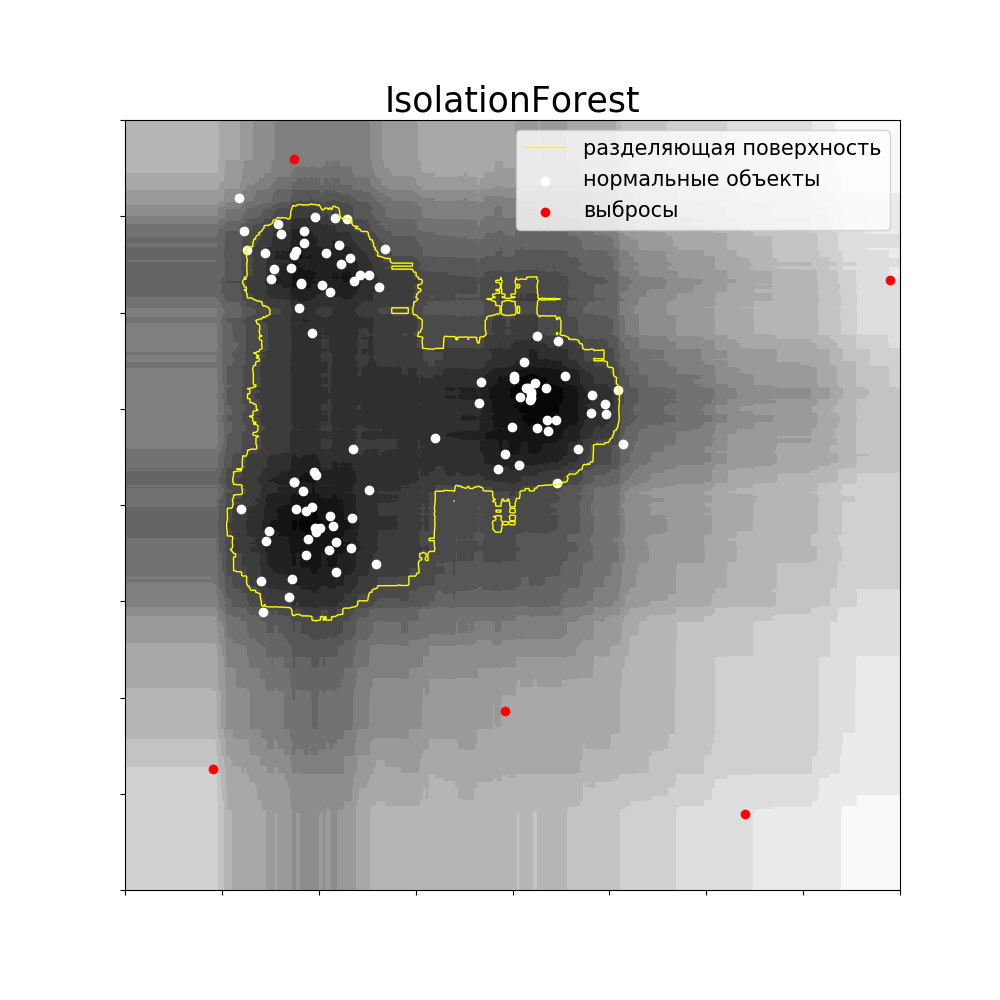
\includegraphics[width=0.3\linewidth]{IsolationForest_3.png}
            \label{sec:Research:Model:Visualization:fig:IsolationForest:3}
        }
        \subfigure[]{
            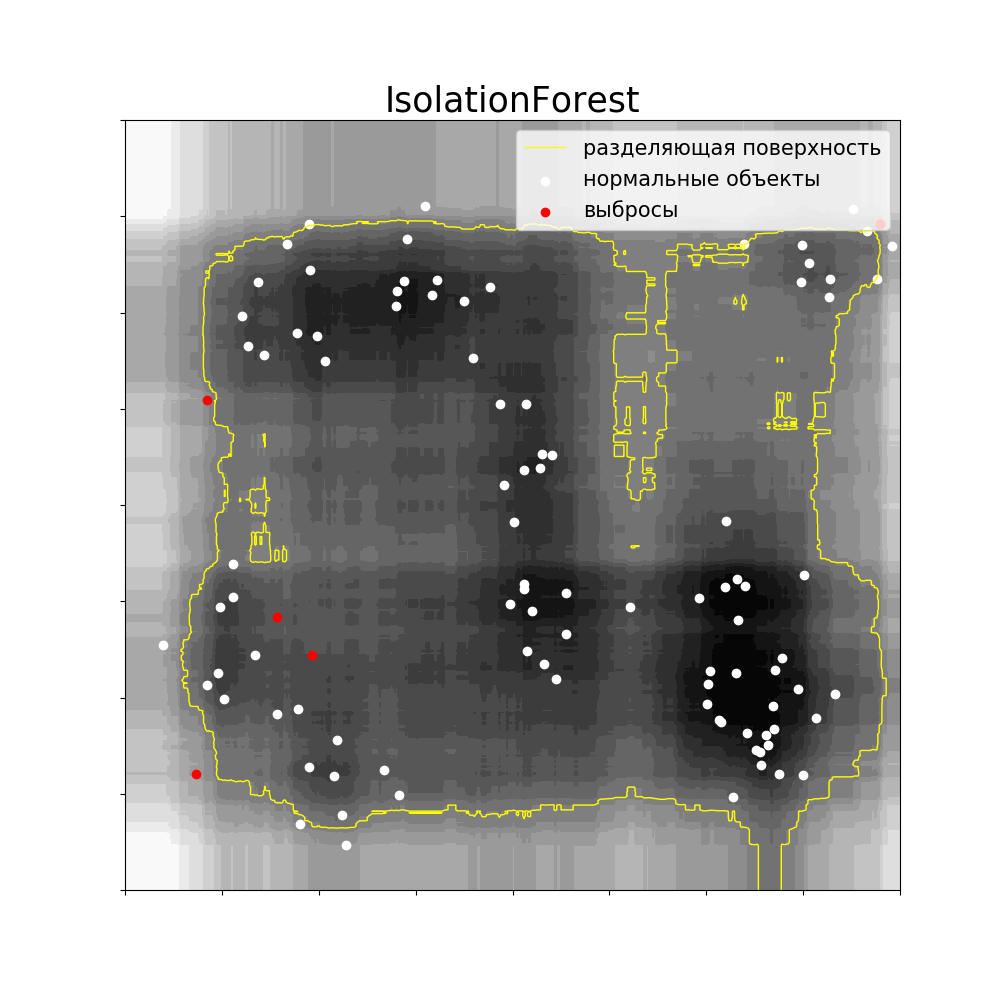
\includegraphics[width=0.3\linewidth]{IsolationForest_10.png}
            \label{sec:Research:Model:Visualization:fig:IsolationForest:10}
        }
        \caption{Isolation Forest: визуализация работы метода на тестовых данных}
        \label{sec:Research:Model:Visualization:fig:IsolationForest}
    \end{figure}

    \par Как видно на рисунке~\ref{sec:Research:Model:Visualization:fig:IsolationForest} изоляционный лес также хорошо проводит разделяющую поверхность.
    \par Алгоритм хорошо отлавливает именно выбросы.

    \newpage


    \textbf{Local Outlier Factor} \\

    \noindent \textsc{Гиперпараметры}
    \begin{itemize}
        \item n\_neighbors -- количество соседей;
        \item contamination – доля выбросов в выборке.
    \end{itemize}

    \noindent \textsc{Достоинства}
    \begin{itemize}
        \item метод способен выявить локальные выбросы в наборе данных.
    \end{itemize}

    \noindent \textsc{Недостатки}
    \begin{itemize}
        \item т.к. метод является метрическим, то он хорошо определяет выбросы только если относительное положение разных точек отражает различие в поведении;
        \item получающиеся значения аномальности труднее интерпретировать.
    \end{itemize}

    % LocalOutlierFactor
    \begin{figure}[h!]
        \centering
        \subfigure[]{
            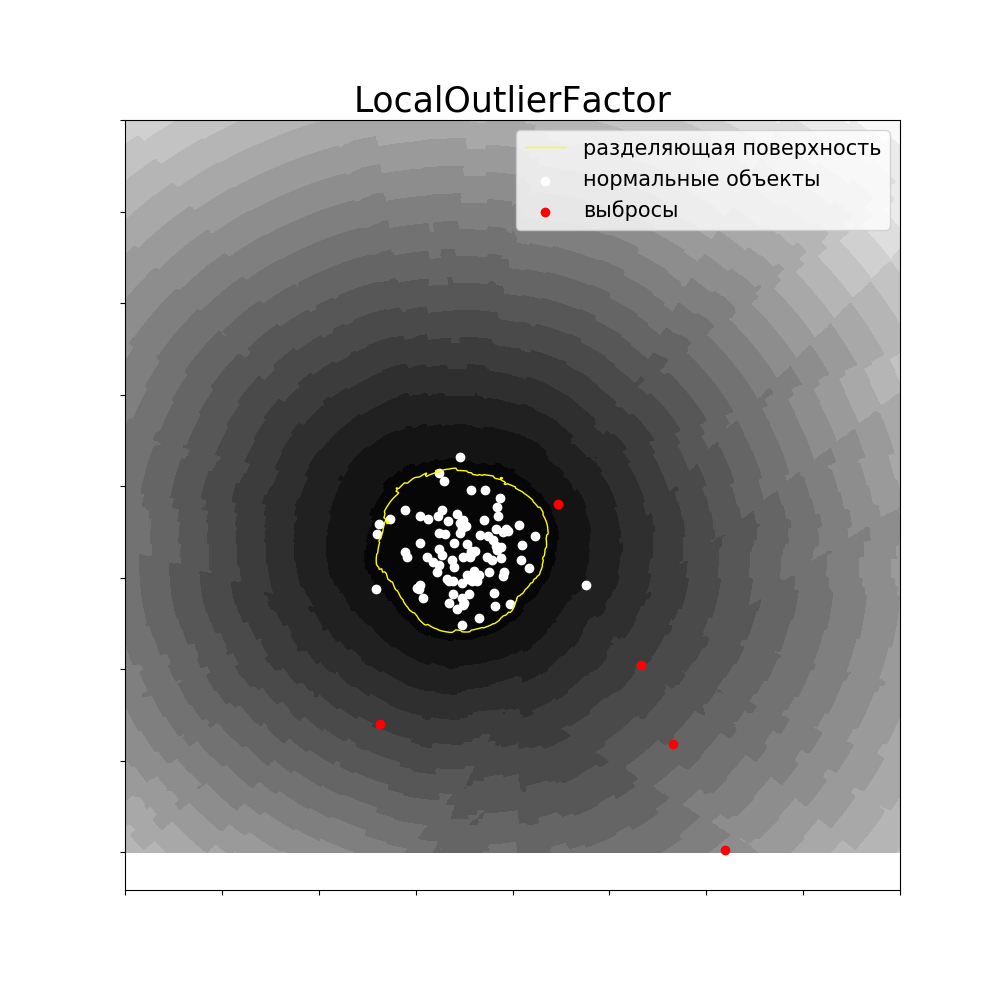
\includegraphics[width=0.3\linewidth]{LocalOutlierFactor_1.png}
            \label{sec:Research:Model:Visualization:fig:LocalOutlierFactor:1}
        }
        \subfigure[]{
            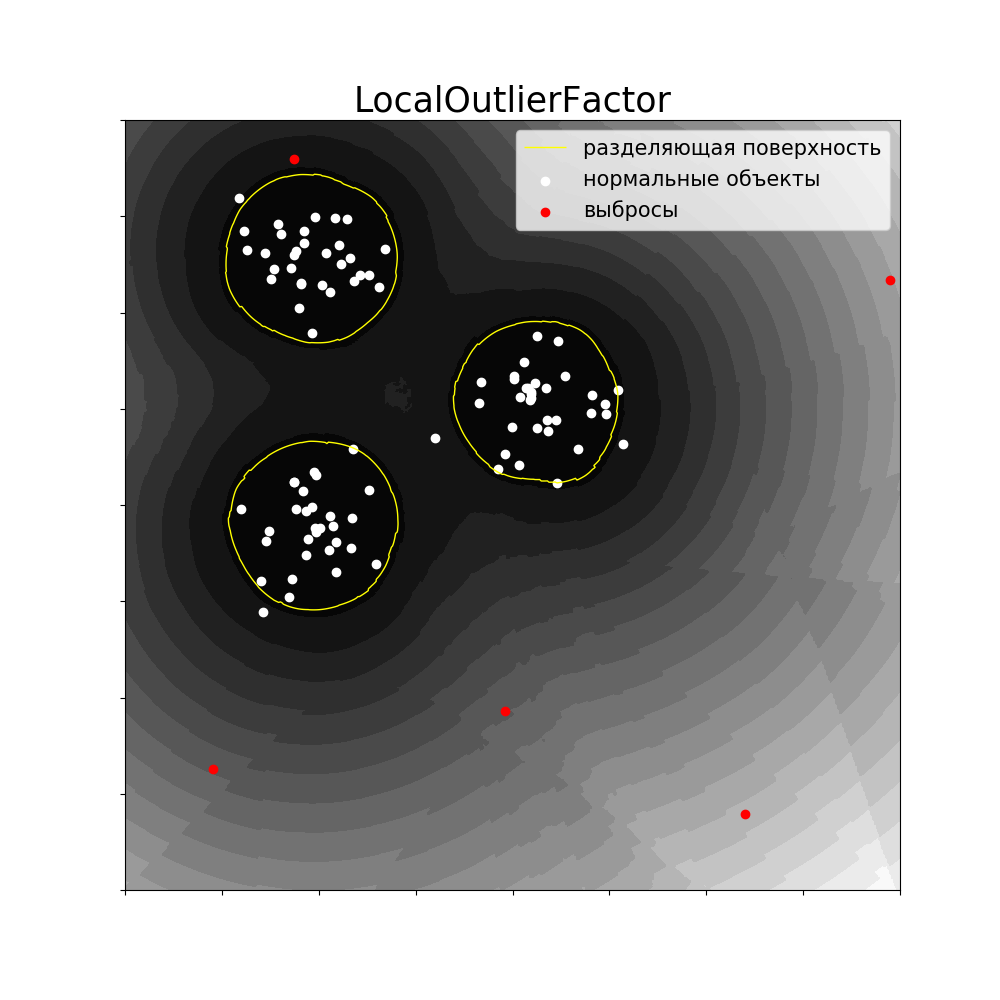
\includegraphics[width=0.3\linewidth]{LocalOutlierFactor_3.png}
            \label{sec:Research:Model:Visualization:fig:LocalOutlierFactor:3}
        }
        \subfigure[]{
            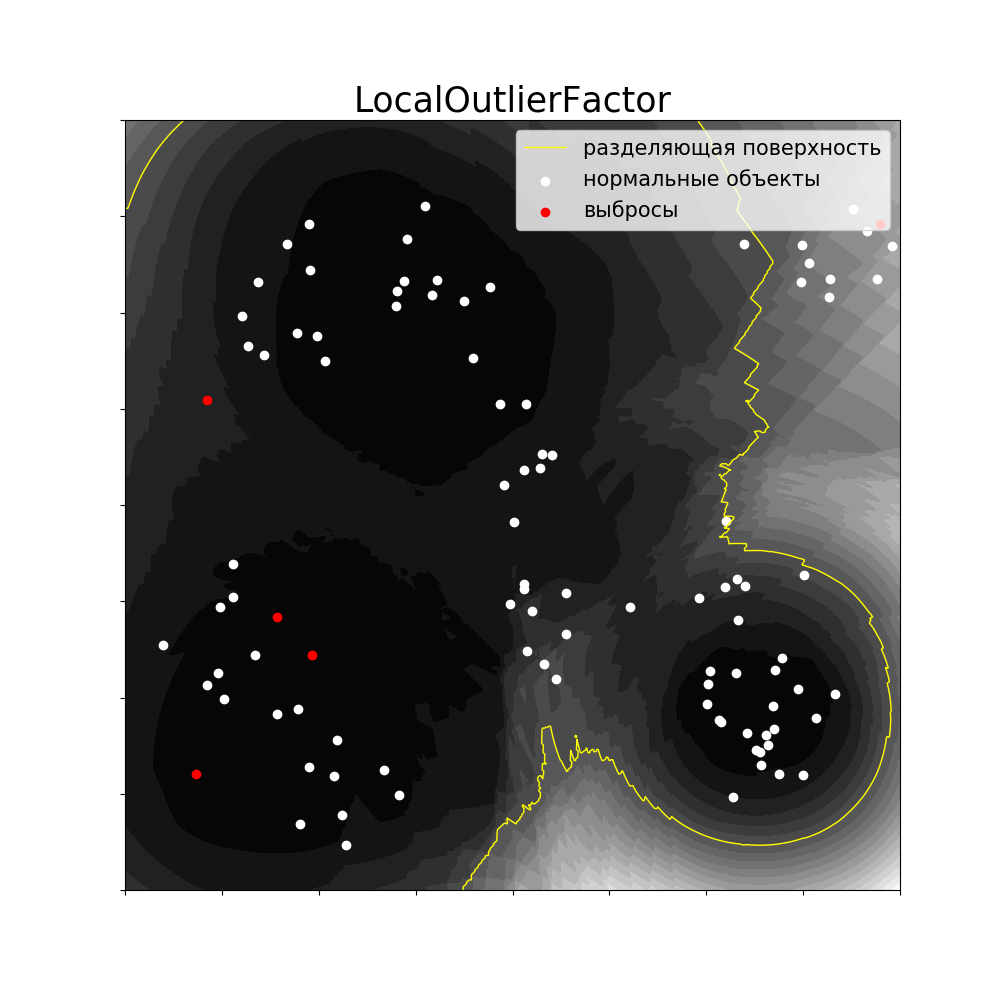
\includegraphics[width=0.3\linewidth]{LocalOutlierFactor_10.png}
            \label{sec:Research:Model:Visualization:fig:LocalOutlierFactor:10}
        }
        \caption{Local Outlier Factor: визуализация работы метода на тестовых данных}
        \label{sec:Research:Model:Visualization:fig:LocalOutlierFactor}
    \end{figure}

    \par Как видно на рисунке~\ref{sec:Research:Model:Visualization:fig:LocalOutlierFactor} алгоритм отлично справляется с поставленной задачей, когда кластеры данных явно выражены. Однако в случае разрозненности наблюдений, как на рисунке \subref{sec:Research:Model:Visualization:fig:LocalOutlierFactor:10}, алгоритм может ошибочно объявить небольшие кластеры наблюдений аномальными.

    \par Мы будем использовать этот метод в качестве предобработки тренировочного набора данных от выбросов.

    \newpage


    \textbf{Elliptic Envelope} \\

    \noindent \textsc{Гиперпараметры}
    \begin{itemize}
        \item contamination – доля выбросов в выборке.
    \end{itemize}

    \noindent \textsc{Достоинства}
    \begin{itemize}
        \item нет необходимости подбирать гиперпараметры модели.
    \end{itemize}

    \noindent \textsc{Недостатки}
    \begin{itemize}
        \item метод успешно работает только на нормально распределенных одномодальных данных.
    \end{itemize}

    % EllipticEnvelope
    \begin{figure}[h!]
        \centering
        \subfigure[]{
            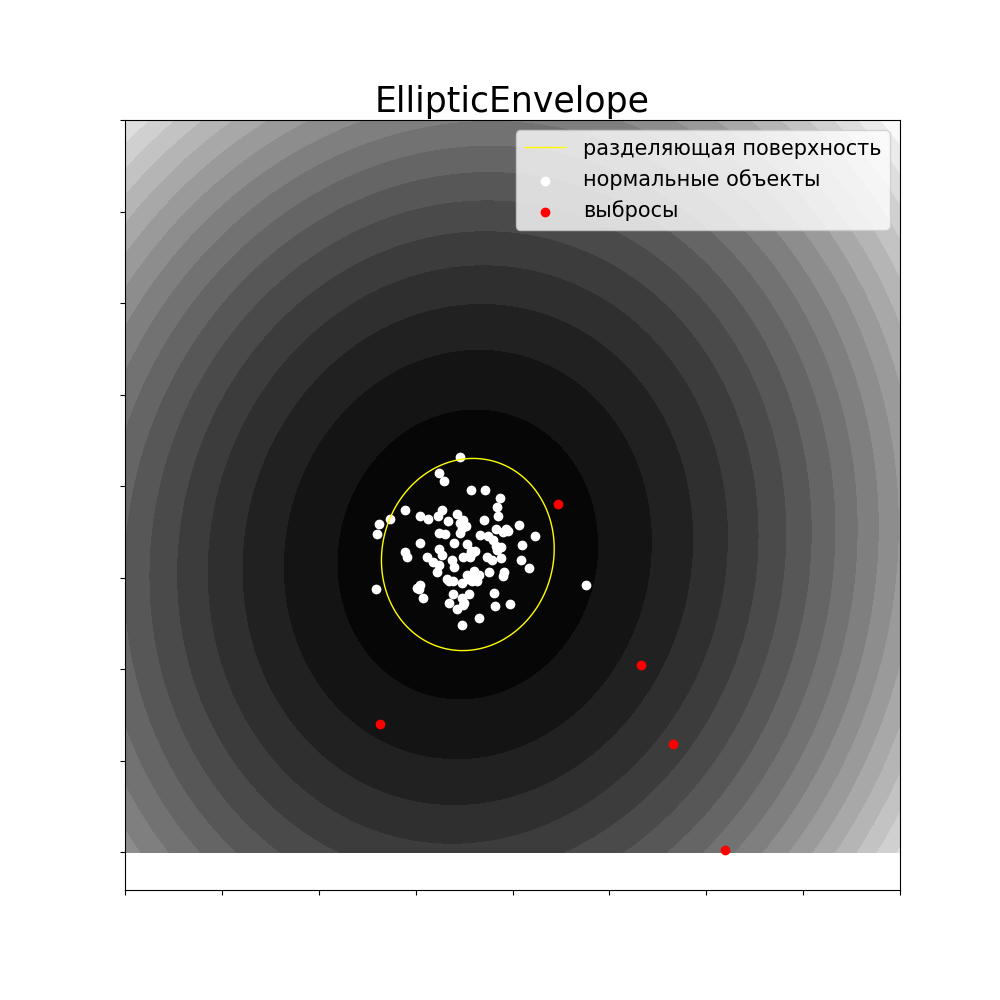
\includegraphics[width=0.3\linewidth]{EllipticEnvelope_1.png}
            \label{sec:Research:Model:Visualization:fig:EllipticEnvelope:1}
        }
        \subfigure[]{
            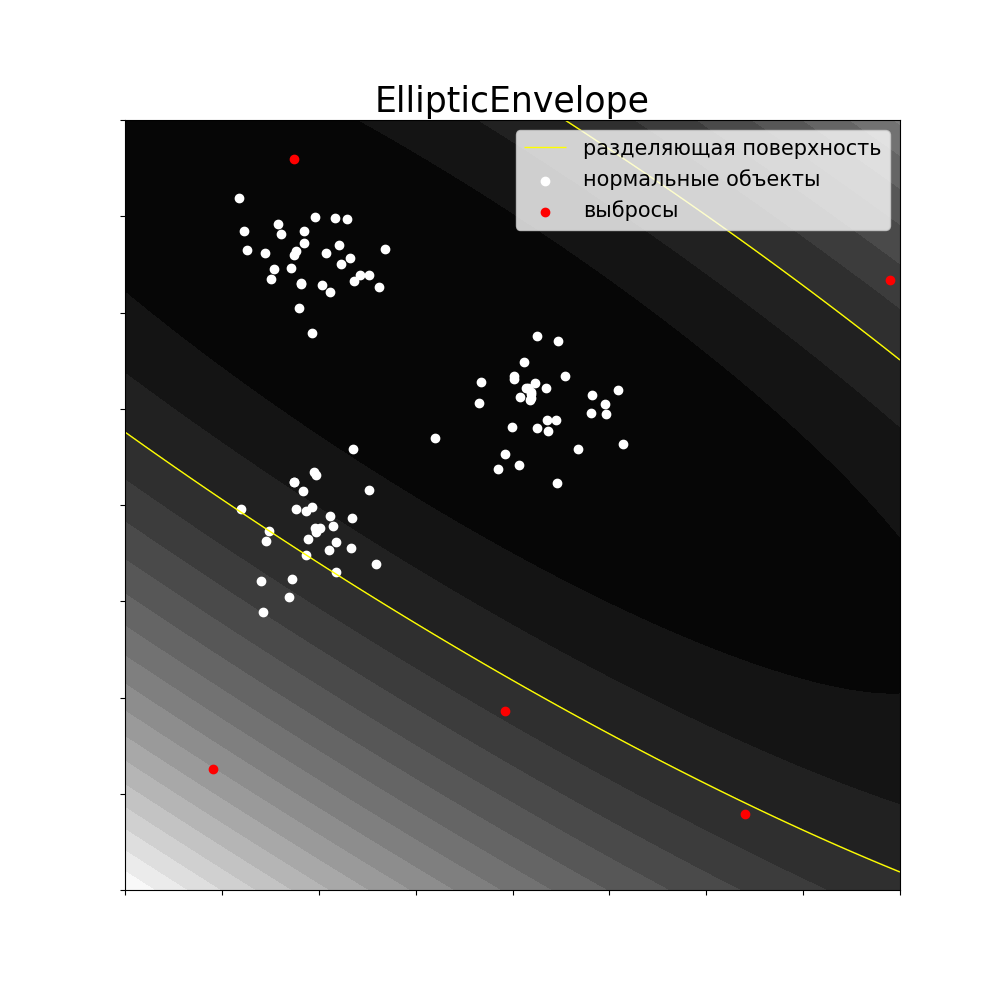
\includegraphics[width=0.3\linewidth]{EllipticEnvelope_3.png}
            \label{sec:Research:Model:Visualization:fig:EllipticEnvelope:3}
        }
        \subfigure[]{
            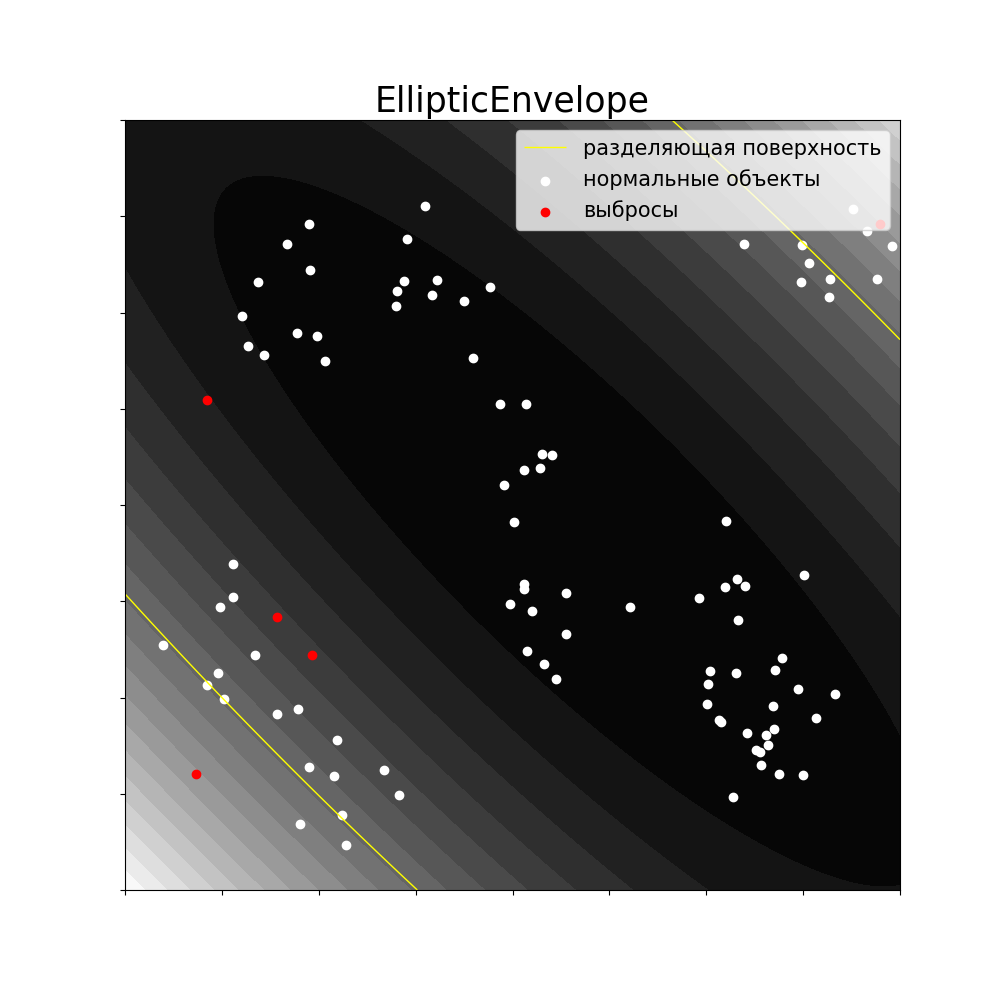
\includegraphics[width=0.3\linewidth]{EllipticEnvelope_10.png}
            \label{sec:Research:Model:Visualization:fig:EllipticEnvelope:10}
        }
        \caption{Elliptic Envelope: визуализация работы метода на тестовых данных}
        \label{sec:Research:Model:Visualization:fig:EllipticEnvelope}
    \end{figure}

    \par На рисунке~\ref{sec:Research:Model:Visualization:fig:EllipticEnvelope} видно, что эллипсоидальная аппроксимация данных работает плохо, если все данные не образуют один локальный кластер. Так на \subref{sec:Research:Model:Visualization:fig:EllipticEnvelope:3} и \subref{sec:Research:Model:Visualization:fig:EllipticEnvelope:10} разделяющая поверхность слишком обширна и охватывает огромную часть пространства, оставив за пределами существенную часть данных.

    \newpage



    \section{Описание практической части}
    \label{sec:PracticalPart}

    \subsection{Программная реализация}
    \label{sec:PracticalPart:Software}

    \par В практической части работы реализован автоматизированный компонентный экспериментальный стенд, архитектура которого представлена на рисунке~\ref{sec:PracticalPart:Software:fig:Architecture}, на языке программирования Python 3 с использованием ряда open source библиотек, основными из которых являются следующие:

    \begin{itemize}
        \item \textsc{Pandas v1.0.0}: для анализа и обработки данных;
        \item \textsc{NumPy v1.18.1}: для эффективной работы с массивами;
        \item \textsc{Scikit-learn v0.22.1}: для решения задач классического машинного обучения;
        \item \textsc{Matplotlib v3.1.3}: для визуализации данных двумерной графикой;
        \item \textsc{Tensorflow v2.1.0}: для решения задач построения и обучения нейронных сетей.
    \end{itemize}

    \begin{figure}[h!]
        \centering
        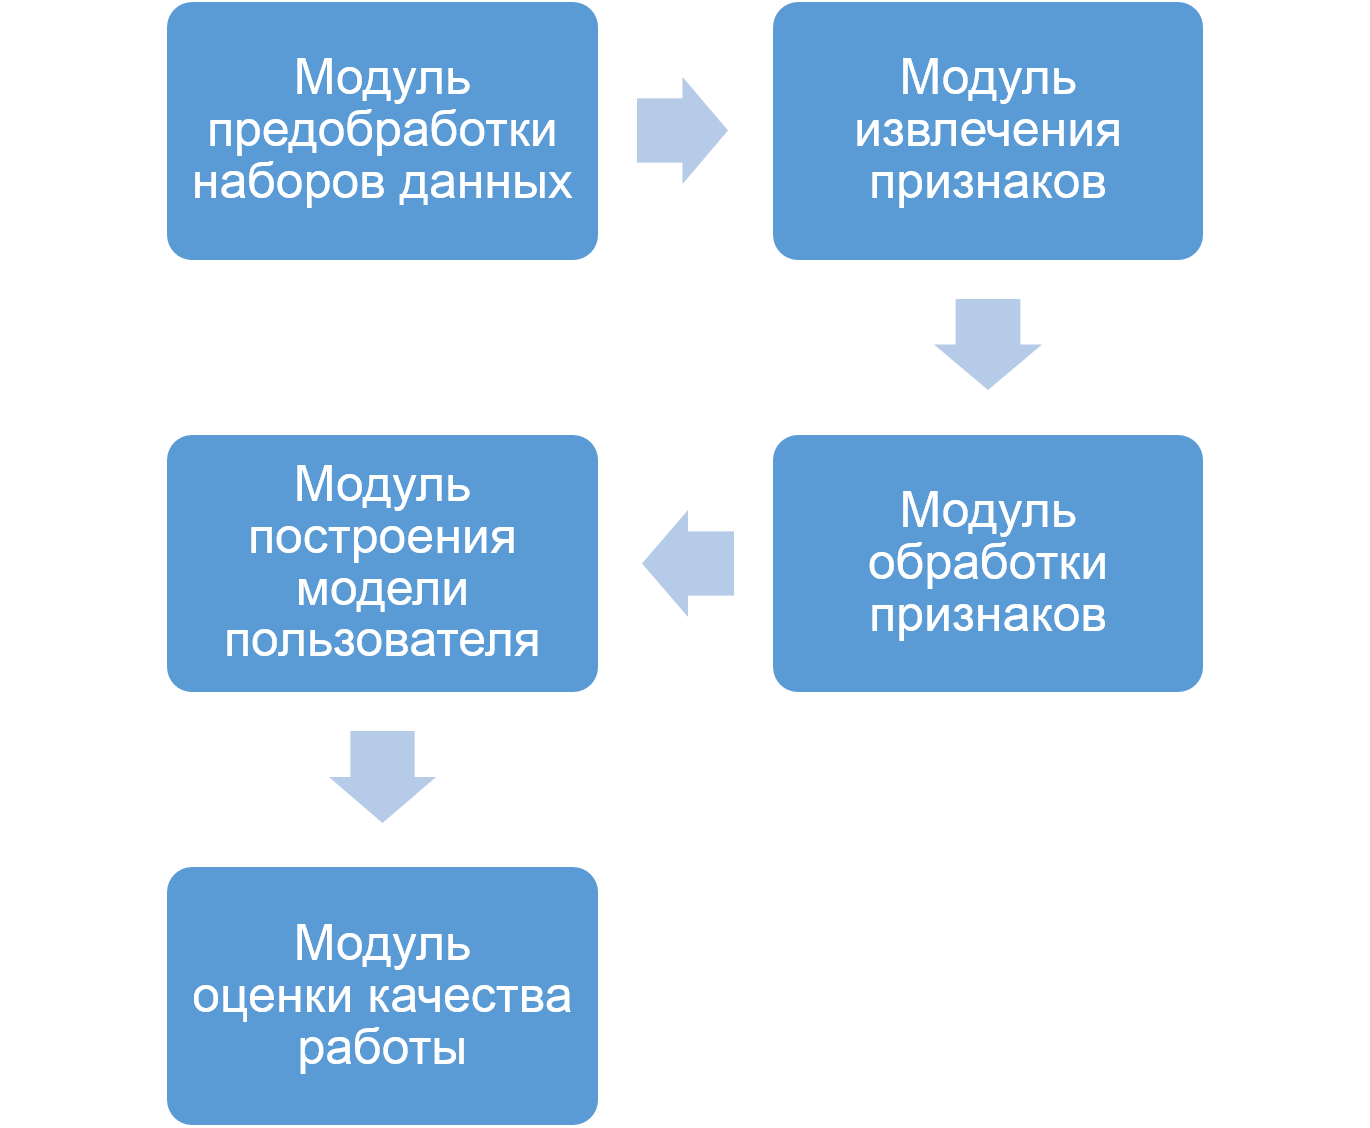
\includegraphics[width=0.9\linewidth]{architecture.png}
        \caption{Архитектура экспериментального стенда}
        \label{sec:PracticalPart:Software:fig:Architecture}
    \end{figure}

    \par \textsc{Модуль предобработки данных}
    \par В рамках данного модуля происходит унифицирование наборов данных, описанных в разделе~\ref{sec:Research:Data:Description}, в соответвии со структурой, заданной в разделе \ref{sec:Research:Data:Struct}. Удаляются все особенности, выявленные в разделе \ref{sec:Research:Data:Features}. Преобразованные наборы данных сохраняются для следующего этапа конвейера. \\

    \par \textsc{Модуль извлечения признаков}
    \par На данном этапе из предобработанных наборов данных происходит выделение признаков, описанных в разделе \ref{sec:Overview:Features} обзора (таблица \ref{sec:Overview:Features:table:FeaturesFormulas} и таблица \ref{sec:Overview:Features:table:ArsFeaturesFormulas}), и сохранение полученных сессий пользователей. \\

    \par \textsc{Модуль обработки признаков}
    \par Далее происходит объединение всех сессий и формирование полного исходного признакового пространства. Также в этом модуле доступны методы предобработки признаковых пространств, описанные в разделе~\ref{sec:Research:FeatureSpace}, результатом работы которых являются модифицированные пространства. \\

    \par \textsc{Модуль построения модели пользователя}
    \par На следующем этапе эксперементального стенда в полученных признаковых пространствах происходит обучение модели пользователя с использованием классических методов машинного обучения, рассмотренных в разделе~\ref{sec:Research:Model}. Подбираются гиперпараметры, при которых модель демонстрирует наилучшее качество работы. Полученные модели сохраняются для возможности дальнейшего использования. \\

    \par \textsc{Модуль оценки качества работы}
    \par В заключительной части происходит оценка качества работы обученных моделей на тестовых наборах данных. Проводится перекрестная проверка one-vs-all, в условиях которой в систему защиты текущего пользователя пытаются проникнуть все остальные пользователи данного набора данных. Усредненное по всем пользователям значение метрики ROC-AUC, описанной в разделе~\ref{sec:Overview:Metrics}, считалось итоговой оценкой качества работы метода. Результатом данного модуля является визуализация оценки качества и сохранение полученных графиков. Пример визуализации качества работы метода во время такой <<атаки>> продемонстрирован на рисунке~\ref{sec:PracticalPart:Software:fig:ROC_curve}. \\

    \par Также в течение работы каждого из описанных модулей ведется подробная запись в log-файлы для сбора статистики и дальнейших исследований. Весь код проекта доступен по ссылке в репозитории: https://github.com/Berezniker/HiddenMouse. Общий объем кода составил порядка TODO.


    \subsection{Экспериментальные исследования}
    \label{sec:PracticalPart:ExperimentalStudy}

    \par В результате работы модуля предобработки были удалены особенности из наборов данных, что составило для каждого пользователя порядка:

    \begin{itemize}
        \item $ 22 \pm 3 \% $ записей в датасете TWOS;
        \item $ 21 \pm 7 \% $ записей в датасете BALABIT; 
        \item $  4 \pm 1 \% $ записей в датасете DATAIIT.
    \end{itemize}

    \par Заметим, что количество неотфильтрованных записей в открытых наборах данных значительно превосходит тот же показатель для датасета, собранного нашей кафедрой в рамках исследования задачи динамической аутентификации пользователя.

    \begin{figure}[h]
        \centering
        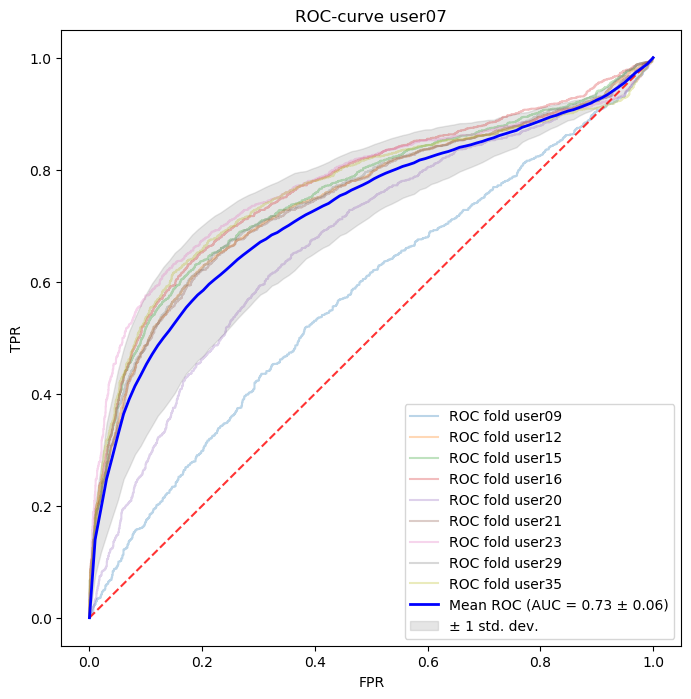
\includegraphics[width=0.85\linewidth]{ROC_curve.png}
        \caption{Пример оценки работы метода}
        \label{sec:PracticalPart:Software:fig:ROC_curve}
    \end{figure}

    \par В модуле извлечения признаков были поставлены эксперименты, результаты которых можно наблюдать в таблице~\ref{sec:PracticalPart:table:TTimeSplit}, с разбиением по временному порогу в T-Time Split разбиении, заданному в разделе \ref{sec:Research:Data:Struct}. Были сделаны следующие выводы:
    \begin{itemize}
        \item $T=1-2$ секунды: долго выделять признаки и обучать модель, мало действий для уникальности одного признака;
        \item $T=3-5$ секунд: \textit{оптимально};
        \item $T=10-15$ секунд: очень быстро, но может оказаться мало векторов для обучения, много действий за один этап;
        \item $T > 15$ секунд: редкая проверка подлинности, пропадает эффект динамики системы, что может стать уязвимостью для внедрения.
    \end{itemize}

    \begin{table}[h]
        \centering
        \caption{Разбиение сессий по временному порогу}
        \begin{tabular}{||c||c||c|c|c|c||}
            \hhline{|t:=:t:=:t:====:t|} 
            \multirow{2}*{Dataset} & \multirow{2}*{Time, h} & \multicolumn{4}{c||}{T-Time Split, sec} \\ \hhline{||~||~||-|-|-|-||}
                                                       & & 2 & 5 & 10 & 15 \\
            \hhline{|:=::=::====:|}
            BALABIT & $43 \pm 17$ & $9600 \pm 4100$ & $4700 \pm 2000$ & $2800 \pm 1200$ & $2000 \pm 800$ \\ \hhline{||-||-||-|-|-|-||}
            DATAIIT & $21 \pm 5$  & $7000 \pm 2500$ & $3400 \pm 1000$ & $2000 \pm 600$  & $1400 \pm 400$ \\ \hhline{||-||-||-|-|-|-||}
            TWOS    & $10 \pm 1$ & $3000\pm 500$ & $1550 \pm 200$ & $800 \pm 100$ & $600 \pm 70$ \\
            \hhline{|b:=:b:=:b:====:b|} 
        \end{tabular}
        \label{sec:PracticalPart:table:TTimeSplit}
    \end{table}

    \par С использованием модуля обработки признаков из предобработанных датасетов были выделены признаки, заданные в таблице \ref{sec:Overview:Features:table:FeaturesFormulas} и таблице \ref{sec:Overview:Features:table:ArsFeaturesFormulas}, описанные в разделе \ref{sec:Overview:Features} обзора. Получившееся признаковое пространство имело размерность 78 признаков на вектор. Также были сформированны модифицированные признаковые пространства в соответвии с методами предобработки, описанными в разделе \ref{sec:Research:FeatureSpace}. В результате чего:

    \begin{itemize}
        \item One-Hot кодировка (раздел \ref{sec:Research:FeatureSpace:OneHotEncoding}) была применена только к корзинным (bin) признакам, что расширило признаковое пространство до 131 признака;
        \item Квантильная дискретизация (раздел \ref{sec:Research:FeatureSpace:Quantile}) была применена ко всем признакам. Построено разбиение на 4 и 10 квантилей.
    \end{itemize}

    \par Перед обучением к исходному тренировочному набору данных было применено преобразование (\ref{sec:PracticalPart:formula:StandartScaler}), стандартизирующее значение всех признаков путем вычитания среднего значения $\mu$ и масштабирования до единичной дисперсии $\sigma$. Преобразование с теми же параметрами было применено в дальнейшем и к тестовому набору.
    \begin{equation}
    \label{sec:PracticalPart:formula:StandartScaler}
        z = \frac{x - \mu}{\sqrt{\sigma}}
    \end{equation}

    \par После чего, на получившихся признаковых пространствах была обучена модель с применением градиентного бустинга (раздел \ref{sec:Research:FeatureSpace:GradientBoostingClassifier}) для выявления наиболее важных признаков.

    \par Результаты экспериментов, представленные в таблице~\ref{sec:PracticalPart:table:Features}, продемонстрировали, что применение One-Hot кодировки и квантильной дискретизации к исходному признаковому пространству не повышает качества аутентификации. Более того, градиентый бустинг показывал низкую значимость почти всех признаков после применения One-Hot кодировки. С учетом того, что эти преобразования увеличивали размерность признакового пространства, что влияло на скорость обучения моделей, было принято решение отказаться от данных модификаций. В свою очередь стандартизация значений (\ref{sec:PracticalPart:formula:StandartScaler}) поспособствовала ускорению и увеличению качества работы методов в среднем на 0.05 по метрике ROC-AUC.

    \par Кроме того, перед обучением модели для динамического обнаружения неконтролируемых локальных выбросов мы применяли технологию Local Outlier Factor, подробно рассмотренную в разделе \ref{sec:Research:Model:LocalOutlierFactor}, что позволило увеличить качество работы методов в среднем на 0.02.

    \begin{table}[h]
        \centering
        \renewcommand{\arraystretch}{1.05}
        \caption{Методы предобработки признакового пространства}
        \begin{tabular}{||c||m{22mm}|m{22mm}|m{22mm}|m{22mm}||c||}
            \hhline{|t:=:t:====:t:=:t|} 
            \multirow{2}*{Модели} & \multicolumn{4}{c||}{Методы предобработки признакового пространства} & \multirow{2}*{ROC-AUC} \\ \hhline{||~||-|-|-|-||~||}
                                  & One-Hot & Quantile & Normalize & Boosting & \\
            \hhline{|:=::====::=:|} 
            \multirow{4}*{OC-SVM} & & & & &          0.0 \\ \hhline{||~||-|-|-|-||-||}
                                  & $\times$ & & & & 0.0 \downarrow \\ \hhline{||~||-|-|-|-||-||}
                                  & & $\times$ & & & 0.0 \downarrow \\ \hhline{||~||-|-|-|-||-||}
                                  & & & $\times$ & & 0.0 \uparrow   \\ \hhline{||~||-|-|-|-||-||}
                                  & & & & $\times$ & 0.0 \uparrow   \\ \hhline{||-||-|-|-|-||-||}
            \multirow{4}*{IF}     & & & & &          0.0 \\ \hhline{||~||-|-|-|-||-||}
                                  & $\times$ & & & & 0.0 \\ \hhline{||~||-|-|-|-||-||}
                                  & & $\times$ & & & 0.0 \\ \hhline{||~||-|-|-|-||-||}
                                  & & & $\times$ & & 0.0 \\ \hhline{||~||-|-|-|-||-||}
                                  & & & & $\times$ & 0.0 \\ \hhline{||-||-|-|-|-||-||}
            \multirow{4}*{LOF}    & & & & &          0.0 \\ \hhline{||~||-|-|-|-||-||}
                                  & $\times$ & & & & 0.0 \\ \hhline{||~||-|-|-|-||-||}
                                  & & $\times$ & & & 0.0 \\ \hhline{||~||-|-|-|-||-||}
                                  & & & $\times$ & & 0.0 \\ \hhline{||~||-|-|-|-||-||}
                                  & & & & $\times$ & 0.0 \\ \hhline{||-||-|-|-|-||-||}
            \multirow{4}*{EE}     & & & & &          0.0 \\ \hhline{||~||-|-|-|-||-||}
                                  & $\times$ & & & & 0.0 \\ \hhline{||~||-|-|-|-||-||}
                                  & & $\times$ & & & 0.0 \\ \hhline{||~||-|-|-|-||-||}
                                  & & & $\times$ & & 0.0 \\ \hhline{||~||-|-|-|-||-||}
                                  & & & & $\times$ & 0.0 \\
            \hhline{|b:=:b:====:b:=:b|} 
        \end{tabular}
        \label{sec:PracticalPart:table:Features}
    \end{table}


    \par Был проведен ряд экспериментов, для выявления наилушего метода из рассмотренных в разделе \ref{sec:Research:Model} методов классического машинного обучения. Для каждой модели были подобраны гиперпараметры, отвечающие наилучшему результату работы метода.

    \begin{table}[h]
        \centering
        \renewcommand{\arraystretch}{1.25}
        \renewcommand{\tabcolsep}{5mm}
        \caption{Гиперпараметры моделей}
        \begin{tabular}{|| c || p{65mm} ||}
            \hhline{|t:=:t:=:t|} 
            Method ML & Hyperparameters \\
            \hhline{|:=::=::|}
            OneClassSVM        & kernel = 'rbf' \newline
                                 gamma = $(n\_features\cdot X.var())^{-1}$ \newline
                                 nu = 0.10 \\ \hhline{||-||-||}
            IsolationForest    & n\_estimators = 10 \newline
                                 max\_samples = 0.7 \newline
                                 contamination = 0.1 \\ \hhline{||-||-||}
            LocalOutlierFactor & n\_neighbors = 10 \newline
                                 algorithm = 'brute' \newline
                                 contaminations = 0.1 \\ \hhline{||-||-||}
            EllipticEnvelope   & support\_fraction = 0.9 \newline
                                 contaminations = 0.1 \\ \hhline{||-||-||}
            \hhline{|b:=:b:=:b|} 
        \end{tabular}
        \label{sec:PracticalPart:table:Hyperparameters}
    \end{table}

    \par Окончательные результаты экспериментов представлены в сводной таблице~\ref{sec:PracticalPart:table:Result}. Как и в обзоре лучшим оказался одноклассовый метод опорных векторов.

    \begin{table}[h]
        \centering
        \renewcommand{\arraystretch}{1.25}
        \renewcommand{\tabcolsep}{5mm}
        \caption{Результаты экспериментальных исследований}
        \begin{tabular}{|| c || c || c | c | c ||}
            \hhline{|t:=:t:=:t:===:t|} 
            Method ML & Dataset & FRR & FAR & ROC-AUC \\
            \hhline{|:=::=::===:|}
            \multirow{3}*{IsolationForest}      & BALABIT & 0.14 & 0.18 & \cellcolor{yellow} 0.68 \\ \hhline{||~||-||-|-|-||}
                                                & DATAIIT & 0.22 & 0.23 & \cellcolor{pink}   0.56 \\ \hhline{||~||-||-|-|-||}
                                                & TWOS    & 0.00 & 0.00 & \cellcolor{white}  0.00 \\ \hhline{||-||-||-|-|-||}
            \multirow{3}*{EllipticEnvelope}     & BALABIT & 0.23 & 0.15 & \cellcolor{yellow} 0.62 \\ \hhline{||~||-||-|-|-||}
                                                & DATAIIT & 0.15 & 0.32 & \cellcolor{pink}   0.53 \\ \hhline{||~||-||-|-|-||}
                                                & TWOS    & 0.00 & 0.00 & \cellcolor{white}  0.00 \\ \hhline{||-||-||-|-|-||}
            \multirow{3}*{\textbf{OneClassSVM}} & BALABIT & 0.14 & 0.15 & \cellcolor{lime}   0.71 \\ \hhline{||~||-||-|-|-||}
                                                & DATAIIT & 0.11 & 0.18 & \cellcolor{lime}   0.80 \\ \hhline{||~||-||-|-|-||}
                                                & TWOS    & 0.00 & 0.00 & \cellcolor{white}  0.00 \\ \hhline{||-||-||-|-|-||}
            \multirow{3}*{LocalOutlierFactor}   & BALABIT & 0.25 & 0.13 & \cellcolor{yellow} 0.60 \\ \hhline{||~||-||-|-|-||}
                                                & DATAIIT & 0.24 & 0.20 & \cellcolor{pink}   0.56 \\ \hhline{||~||-||-|-|-||}
                                                & TWOS    & 0.00 & 0.00 & \cellcolor{white}  0.00 \\
            \hhline{|b:=:b:=:b:===:b|} 
        \end{tabular}
        \label{sec:PracticalPart:table:Result}
    \end{table}

    \newpage



    \section{Планы на будущее}
    \label{sec:Future}

    \par Нейронные сети активно применяются в сфере безопасности. Они работают быстрее и показывают результат лучше классических методов машинного обучения. Поэтому дальнейшие исследования будут направлены на поиск решения поставленной задачи с применением нейронных сетей.

    \par Решение о легитимности пользователя предложено принимать на основе сравнения с пороговым значением результата работы функции оценки предсказания модели по заданному биометрическому набору данных с векторами признаков из тренировочного набора данных.

    \par Исследования в этом направление уже ведутся.


    \subsection{Автокодировщик}
    \label{sec:Future:Autoencoder}

    \par Автокодировщик (autoencoder) \cite{autoencoder} -- это нейронная сеть, которая восстанавливает входной сигнал на выходе. Автокодировщик состоит из двух частей: кодировщика, который кодирует данные в свое внутреннее представление, и декодировщика, который восстанавливает исходный вектор. Обычно автокодировщики ограничивают в размерности скрытых слоев (они меньше, чем размерность сигнала на входе) и используют l1-, l2-регуляризаторы для штрафов за активации в скрытых слоях.

    \begin{figure}[h!]
        \centering
        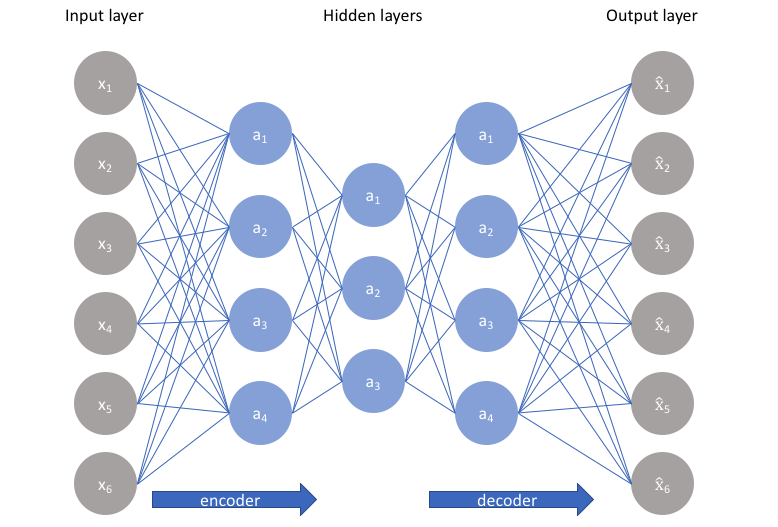
\includegraphics[width=0.9\linewidth]{autoencoder.png}
        \caption{Архитектура сети автокодировщика}
        \label{sec:Future:autoencoder:fig:autoencoder}
    \end{figure}


    \subsection{Рекуррентные нейронные сети}
    \label{sec:Future:LSTM}

    \par Одним из преимуществ рекуррентных нейросетей (RNN: Recurrent Neural Networks) \cite{RNN} является тот факт, что они потенциально умеют связывать информацию с предыдущих входных значений с текущим вектором признаков. Рекуррентные нейронные сети содержат обратные связи.

    \par Долгая краткосрочная память (LSTM: Long Short-Term Memory) \cite{LSTM} – особый вид архитектуры рекуррентных нейронных сетей, способный к обучению долговременных связей.

    \begin{figure}[h!]
        \centering
        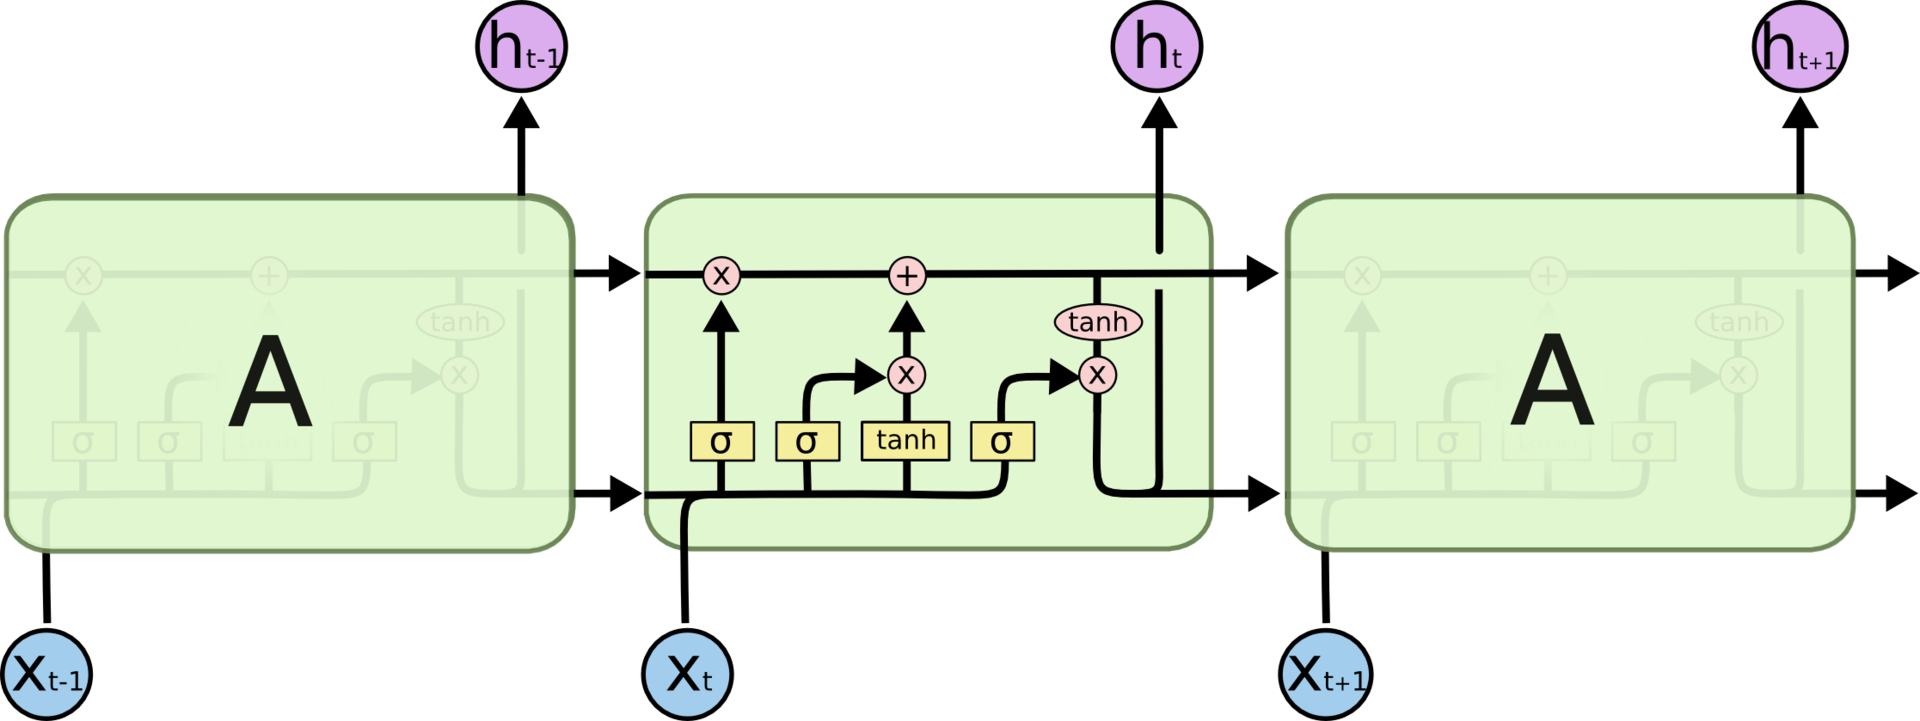
\includegraphics[width=0.9\linewidth]{LSTM.png}
        \caption{Структура нейрона с LSTM}
        \label{sec:Future:LSTM:fig:LSTM}
    \end{figure}


    \subsection{Полносверточные нейронные сети}
    \label{sec:Future:FCNN}

    \par Основной особенностью полносверточных нейросетей \cite{FCNN} (FCNN: Fully Convolutional Neural Network) является относительно небольшое число параметров за счет использования сверточных слоев, что позволяет конструировать и обучать более сложные архитектуры для повышения качества решения поставленной задачи.

    \begin{figure}[h!]
        \centering
        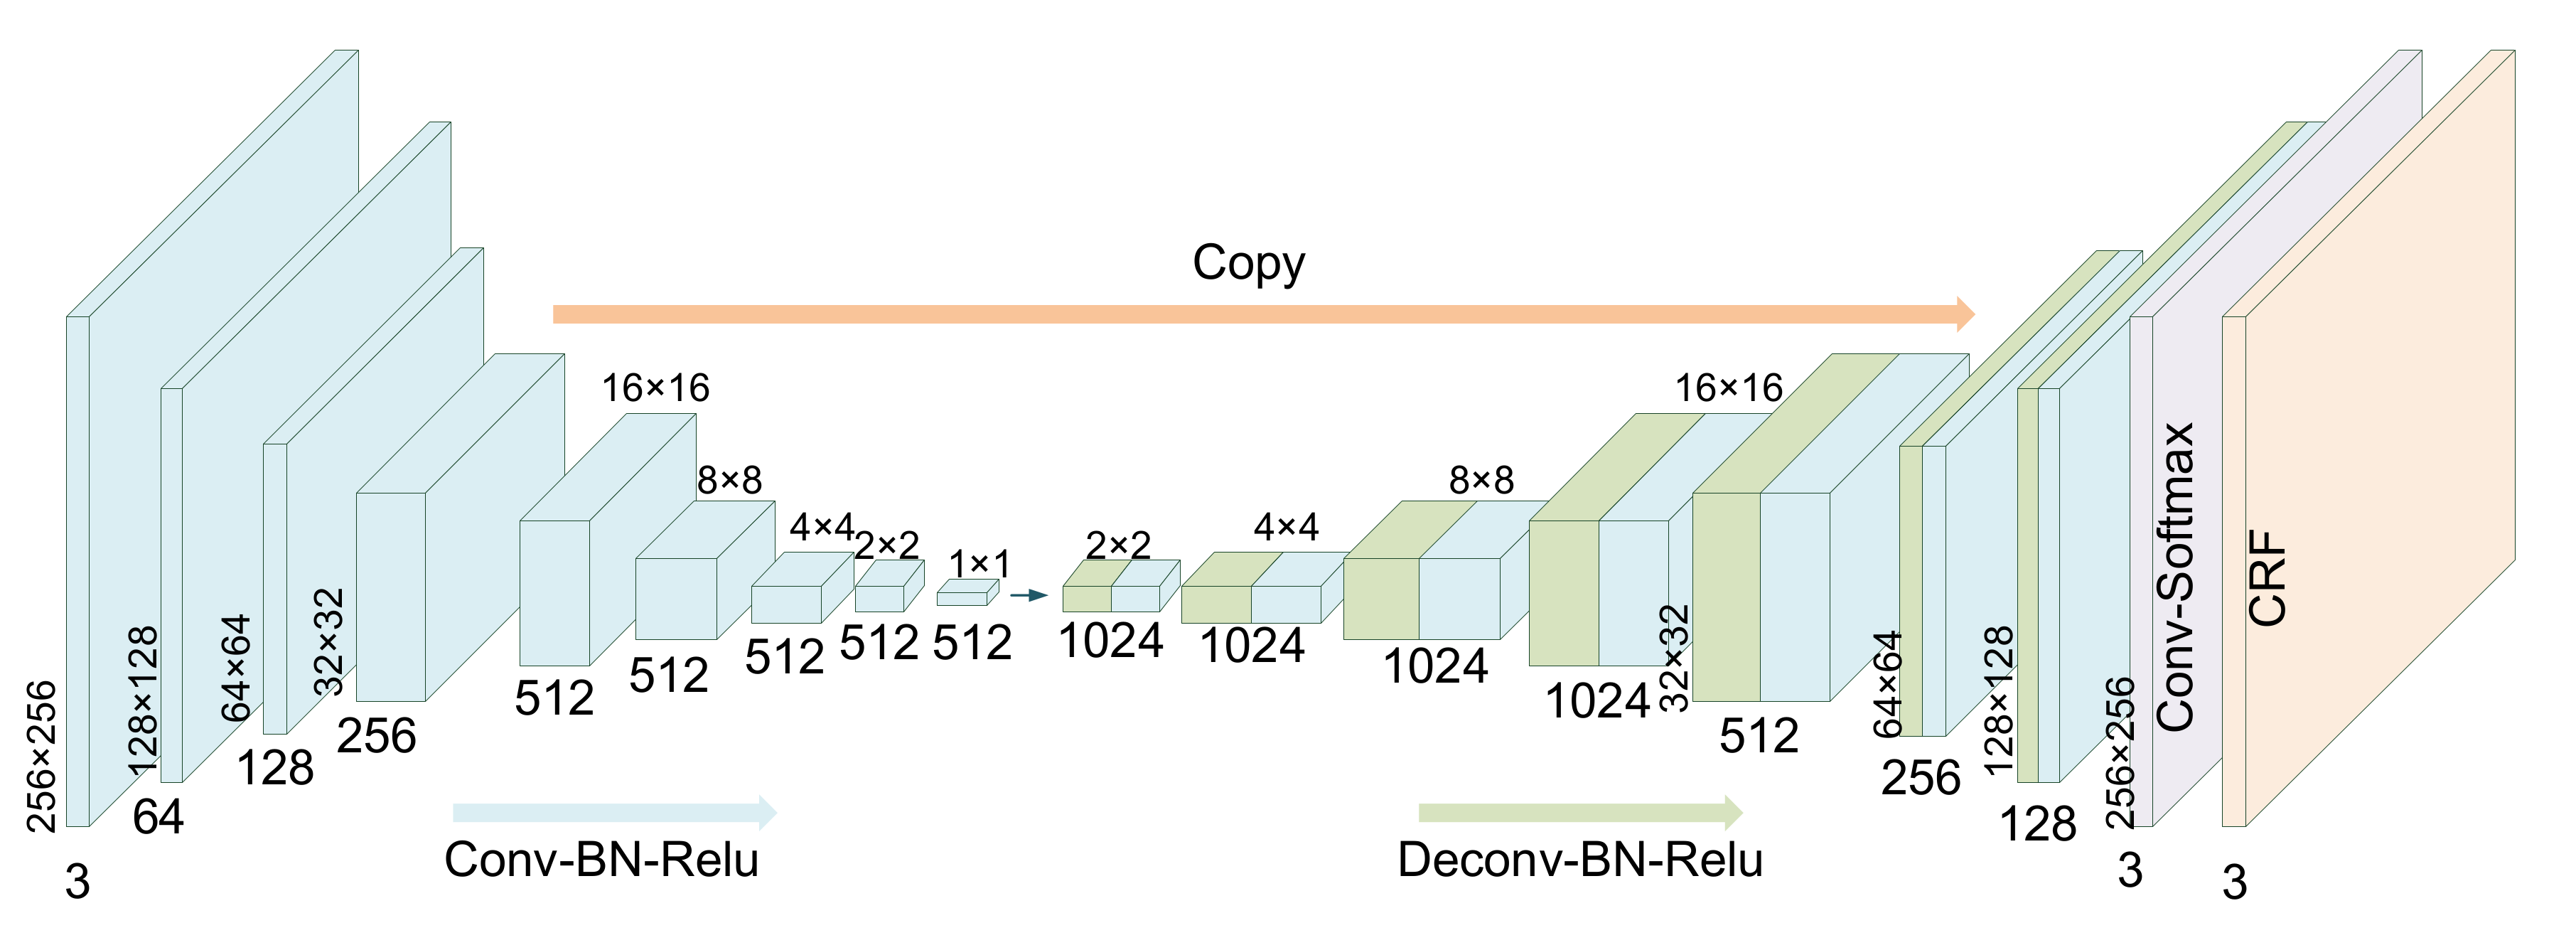
\includegraphics[width=0.9\linewidth]{FCNN.png}
        \caption{Архитектура полносверточного автокодировщика}
        \label{sec:Future:FCNN:fig:FCNN}
    \end{figure}

    \newpage



    \section{Заключение}
    \label{sec:Conclusion}

    \par В рамках данной работы выполнены все поставленные задачи:

    \begin{itemize}
        \item рассмотрены существующие методы решения задачи динамической аутентификации пользователя на основе анализа его работы с компютерной мышью с использованием классических методов машинного обучения;
        \item рассмотрены способы построения признаковых пространств, описывающих динамику работы пользователя с компьютерной мышью, и методы предобработки получившихся вектор-признаков;
        \item предложены модификации алгоритмов для повышения качества работы методов;
        \item разработан компонентный экспериментальный стенд и проведены исследдования для подтверждения гипотезы об улучшения качества работы методов с предложенными модификациями.
    \end{itemize}

    \newpage



    \begin{thebibliography}{20}
        \bibitem{BiometricRecognition}
        Jain A. K., Ross A., Prabhakar S. An introduction to biometric recognition //IEEE Transactions on circuits and systems for video technology. – 2004. – Т. 14. – №. 1. – С. 4-20.

        \bibitem{BiometricSystem}
        Wayman J. et al. An introduction to biometric authentication systems //Biometric Systems. – Springer, London, 2005. – С. 1-20.

        \bibitem{BoiometricSecurity}
        John D. Cook Biometric security and hypothesis testing (https://www.johndcook.com/blog/2018/10/31/biometric-security-error/)

        \bibitem{Mondal}
        Mondal S., Bours P. A study on continuous authentication using a combination of keystroke and mouse biometrics //Neurocomputing. – 2017. – Т. 230. – С. 1-22.

        \bibitem{Mondal_2}
        Mondal S., Bours P. Combining keystroke and mouse dynamics for continuous user authentication and identification //2016 IEEE International Conference on Identity, Security and Behavior Analysis (ISBA). – IEEE, 2016. – С. 1-8

        \bibitem{Mondal_3}
        Mondal S., Bours P. A computational approach to the continuous authentication biometric system //Information Sciences. – 2015. – Т. 304. – С. 28-53.

        \bibitem{Stokes}
        Stokes R. et al. Comparison of Biometric Authentication Software Techniques: GEFE vs. Angle Based Metrics //MAICS. – 2016. – С. 75-89.

        \bibitem{Antal}
        Antal M., Egyed-Zsigmond E. Intrusion detection using mouse dynamics //IET Biometrics. – 2019.

        \bibitem{Fridman}
        Fridman L. et al. Multi-modal decision fusion for continuous authentication //Computers & Electrical Engineering. – 2015. – Т. 41. – С. 142-156.

        \bibitem{Khalifa}
        Khalifa A. A. et al. Comparison between mixed binary classification and voting technique for active user authentication using mouse dynamics //2015 International Conference on Computing, Control, Networking, Electronics and Embedded Systems Engineering (ICCNEEE). – IEEE, 2015. – С. 281-286.

        \bibitem{Masri}
        El Masri A. et al. Active authentication using scrolling behaviors //2015 6th International Conference on Information and Communication Systems (ICICS). – IEEE, 2015. – С. 257-262.

        \bibitem{Borisov}
        Борисов Р. В. и др. Оценка идентификационных возможностей особенностей работы пользователя с компьютерной мышью //Вестник Сибирской государственной автомобильно-дорожной академии. – 2015. – №. 5 (45).

        \bibitem{Kasprowski}
        Kasprowski P., Harezlak K. Biometric Identification Using Gaze and Mouse Dynamics During Game Playing //International Conference: Beyond Databases, Architectures and Structures. – Springer, Cham, 2018. – С. 494-504.

        \bibitem{Tan}
        Tan Y. X. M., Binder A., Roy A. Insights from curve fitting models in mouse dynamics authentication systems //2017 IEEE Conference on Application, Information and Network Security (AINS). – IEEE, 2017. – С. 42-47.

        \bibitem{Shen}
        Shen C. et al. Pattern-growth based mining mouse-interaction behavior for an active user authentication system //IEEE Transactions on Dependable and Secure Computing. – 2017.

        \bibitem{Pilankar}
        Pilankar P. S., Padiya P. Multi-phase mouse dynamics authentication system using behavioural biometrics //2016 International Conference on Signal Processing, Communication, Power and Embedded System (SCOPES). – IEEE, 2016. – С. 1947-1950.

        \bibitem{Chong}
        Chong P., Elovici Y., Binder A. User Authentication Based on Mouse Dynamics Using Deep Neural Networks: A Comprehensive Study //IEEE Transactions on Information Forensics and Security. – 2019.

        \bibitem{Chong2D}
        Chong P. et al. Mouse Authentication without the Temporal Aspect–What does a 2D-CNN learn? //2018 IEEE Security and Privacy Workshops (SPW). – IEEE, 2018. – С. 15-21.
        
        \bibitem{Monaro}
        Monaro M., Gamberini L., Sartori G. The detection of faked identity using unexpected questions and mouse dynamics //PloS one. – 2017. – Т. 12. – №. 5. – С. e0177851.

        \bibitem{ArsFeature}
        Feher C. et al. User identity verification via mouse dynamics //Information Sciences. – 2012. – Т. 201. – С. 19-36.

        \bibitem{BALABIT}
        Fülöp, Á., Kovács, L., Kurics, T., Windhager-Pokol, E. (2016). Balabit Mouse Dynamics Challenge data set. Available at: https://github.com/balabit/Mouse-Dynamics-Challenge

        \bibitem{TWOS}
        Harilal A. et al. Twos: A dataset of malicious insider threat behavior based on a gamified competition //Proceedings of the 2017 International Workshop on Managing Insider Security Threats. – 2017. – С. 45-56.

        \bibitem{GBM}
        Friedman J. H. Greedy function approximation: a gradient boosting machine //Annals of statistics. – 2001. – С. 1189-1232.

        \bibitem{BINNING}
        Binning [HTML] (https://wiki.loginom.ru/articles/binning.html)

        \bibitem{Kazachuk}
        Kazachuk M. et al. One-class models for continuous authentication based on keystroke dynamics //International Conference on Intelligent Data Engineering and Automated Learning. – Springer, Cham, 2016. – С. 416-425.

        \bibitem{Dyakonov}
        Дьяконов А.Г. Поиск аномалий (Anomaly Detection) (https://dyakonov.org/2017/04/19/поиск-аномалий-anomaly-detection/)

        \bibitem{NoveltyDetection}
        Pimentel M. A. F. et al. A review of novelty detection //Signal Processing. – 2014. – Т. 99. – С. 215-249.

        \bibitem{SVM}
        Cortes C., Vapnik V. Support-vector networks //Machine learning. – 1995. – Т. 20. – №. 3. – С. 273-297.

        \bibitem{OC-SVM}
        Manevitz L. M., Yousef M. One-class SVMs for document classification //Journal of machine Learning research. – 2001. – Т. 2. – №. Dec. – С. 139-154.

        \bibitem{IsolationForest}
        Liu F. T., Ting K. M., Zhou Z. H. Isolation forest //2008 Eighth IEEE International Conference on Data Mining. – IEEE, 2008. – С. 413-422.

        % \bibitem{IsolationForest_2}
        % Eryk Lewinson Outlier Detection with Isolation Forest [HTML] (https://towardsdatascience.com/outlier-detection-with-isolation-forest-3d190448d45e)

        % \bibitem{IsolationForeset_3}
        % Adithya Krishnan Anomaly Detection with Isolation Forest \& Visualization (https://towardsdatascience.com/anomaly-detection-with-isolation-forest-visualization-23cd75c281e2)

        \bibitem{LOF}
        Breunig M. M. et al. LOF: identifying density-based local outliers //Proceedings of the 2000 ACM SIGMOD international conference on Management of data. – 2000. – С. 93-104.

        % \bibitem{LOF_2}
        % Christopher Jose Anomaly Detection Techniques in Python (https://medium.com/learningdatascience/anomaly-detection-techniques-in-python-50f650c75aaf)

        \bibitem{EE}
        Hoyle B. et al. Anomaly detection for machine learning redshifts applied to SDSS galaxies //Monthly Notices of the Royal Astronomical Society. – 2015. – Т. 452. – №. 4. – С. 4183-4194.

        \bibitem{autoencoder}
        Ng A. et al. Sparse autoencoder //CS294A Lecture notes. – 2011. – Т. 72. – №. 2011. – С. 1-19.

        \bibitem{RNN}
        Rumelhart D. E., Hinton G. E., Williams R. J. Learning internal representations by error propagation. – California Univ San Diego La Jolla Inst for Cognitive Science, 1985. – №. ICS-8506.

        \bibitem{LSTM}
        Hochreiter S., Schmidhuber J. Long short-term memory //Neural computation. – 1997. – Т. 9. – №. 8. – С. 1735-1780.

        % \bibitem{LSTM_2}
        % Christopher Olah Understanding LSTM Networks (http://colah.github.io/posts/2015-08-Understanding-LSTMs/)

        \bibitem{FCNN}
        Long J., Shelhamer E., Darrell T. Fully convolutional networks for semantic segmentation //Proceedings of the IEEE conference on computer vision and pattern recognition. – 2015. – С. 3431-3440.

    \end{thebibliography}


\end{document}
